    \documentclass[12pt]{article}
    \usepackage{amsmath,amsthm,epsfig,graphicx}
    \usepackage{enumerate}
    %\usepackage{jf}                 % JF style to reference
    \usepackage{setspace}          % doublespace
    \usepackage{amsfonts}
    \usepackage{float}
    \usepackage{natbib}
    \usepackage{url}
    \usepackage{hyperref}
    \usepackage{xcolor}
    \usepackage{booktabs}
    \usepackage{pdflscape}  
    \usepackage[T1]{fontenc}
    \usepackage{xr}
    \externaldocument{main}
     \usepackage[font=small,labelfont=bf,tableposition=top]{caption}
     \DeclareCaptionLabelFormat{andtable}{#1~#2  \&  \tablename~\thetable}
     
     


    \setlength{\textwidth}{6.2in} \setlength{\textheight}{9.2in}
    \setlength{\evensidemargin}{.25in}
    \setlength{\oddsidemargin}{\evensidemargin}
    \setlength{\topmargin}{0.25in} \setlength{\headheight}{0in}
    \setlength{\headsep}{0in} \setlength{\topskip}{0in}
    \setlength{\parskip}{0cm}
    
    
    
    
    

    \renewcommand{\baselinestretch}{1.5}  % linespacing, 2 doublespace
    \parskip 3pt          % sets spacing between paragraphs
   \parindent 15pt         % sets leading space for paragraphs, 0=noindent

    \theoremstyle{plain}
\newtheorem{lemma}{Lemma} 
\newtheorem{theorem}{Theorem}
\newtheorem{prop}{Proposition} 
\newtheorem{corollary}{Corollary}
\newtheorem{defn}{Definition}
\newtheorem{exam}{Example}
\newtheorem{rmk}{Remark}

\newcommand{\olpi}{\overline{\pi}}
\newcommand{\ulpi}{\underline{\pi}}


    \usepackage{multirow}
    \usepackage{array}
    \usepackage{changepage}
    \newcommand{\w}{1.5cm}


\renewcommand{\thesection}{\Roman{section}}
\renewcommand{\thesubsection}{\Alph{subsection}}
\newcommand{\bfsym}[1]{\boldsymbol{#1}}               
\renewcommand{\labelenumi}{(\theenumi)}                 % changes style of first layer of eunmerate
\renewcommand{\theenumi}{\roman{enumi}}                 % changes first layer of enumerate environment
\renewcommand{\labelenumii}{(\theenumi)(\theenumii)}   % changes style of second layer of eunmerate
\renewcommand{\theenumii}{\alph{enumii}}                % changes second layer of enumerate environment

\newcommand{\halfskip}{\vskip 0.5\baselineskip}

\begin{document}


\begin{titlepage}

  \singlespace \newcounter{tmark} \setcounter{tmark}{1}
  \renewcommand{\thefootnote}{\fnsymbol{footnote}}
\title{Internet Appendix for \\ ``Demand Disagreement"}

\end{titlepage}

    \date{\today}
\maketitle



This Internet Appendix serves as a companion to our paper ``Demand Disagreement.'' It provides additional results and proofs not reported in the main text due to space constraints. 

\begin{enumerate}
 \item Empirical Results
 \item Unscented Kalman Filter (UKF)
 \item Using yield forecast disagreement and macro disagreement in the UKF
 \item Alternative Calibration
 \item Reverse False Consensus Bias
 \item General disagreement
 \item Production economy
 \item Wealth Shares
 \item Correlation Puzzle
 \item Price-dividend ration and return predictability
 \item Changes in demand risk exposure
 \item Black's leverage effect
\end{enumerate}


\section{Empirical Results}\label{IAempirics}
In this section we present some additional results and robustness checks. 
\subsection{Disagreement Spanning Regressions}
In the main text we report the $R^2$ from the disagreement spanning regressions. Here we include information on the coefficients and t-stat for the regressions. 

\begin{table}[H]
\centering
\caption{Definitions of Variables from the Survey of Professional Forecasters}
\begin{tabular}{p{2.5cm} p{10cm}}
\hline
\hline
\textbf{Variable} & \textbf{Definition} \\
\hline
BOND & Forecasts for the quarterly average and annual-average level of Moody’s Aaa corporate bond yield. \\
CPI & Consumer Price Index, measuring the average change over time in prices paid by urban consumers for a market basket of goods and services. \\
HOUSING & Housing starts, representing the number of new residential construction projects begun during a specific period. \\
UNEMP & Unemployment rate, indicating the percentage of the labor force that is jobless and actively seeking employment. \\
gCPROF & Forecasted growth rate of corporate profits. \\
gRCONSUM & Forecasted growth rate of real personal consumption expenditures, reflecting consumer spending adjusted for inflation. \\
gRFEDGOV & Forecasted growth rate of real federal government consumption expenditures and gross investment, adjusted for inflation. \\
gRGDP & Forecasted growth rate of real Gross Domestic Product, measuring the value of economic output adjusted for inflation. \\
gRNRESIN & Forecasted growth rate of real nonresidential fixed investment, indicating business investments in structures, equipment, and software, adjusted for inflation. \\
gRRESINV & Forecasted growth rate of real residential fixed investment, representing investments in residential structures, adjusted for inflation. \\
\hline
\hline
\end{tabular}
\end{table}


\subsubsection{Baseline regressions}
\begin{table}[H]
\centering
\caption{Regression Results: Level Specifications}
\begin{tabular}{@{\extracolsep{5pt}}lcccc}
\hline
\hline
& (1) & (2) & (3) & (4) \\
\hline
BOND & 0.659$^{***}$ & 0.984$^{***}$ & 0.934$^{***}$ & 0.827$^{***}$ \\
     & (0.099) & (0.090) & (0.082) & (0.085) \\

CPI  & 0.016 & -0.016 & 0.116$^{**}$ & 0.200$^{***}$ \\
     & (0.032) & (0.039) & (0.047) & (0.062) \\

HOUSING & -0.087 & -0.168 & -0.657 & -1.256$^{**}$ \\
        & (0.598) & (0.523) & (0.508) & (0.533) \\

UNEMP & -0.406$^{***}$ & -0.467$^{***}$ & -0.335$^{***}$ & -0.229$^{**}$ \\
      & (0.080) & (0.080) & (0.080) & (0.089) \\

gCPROF & -0.013 & 0.462$^{*}$ & 1.339$^{***}$ & 2.352$^{***}$ \\
       & (0.178) & (0.268) & (0.412) & (0.666) \\

gRCONSUM & 3.734$^{**}$ & 3.143 & -0.613 & -4.935 \\
         & (1.743) & (2.691) & (2.874) & (3.585) \\

gRFEDGOV & 0.837 & -1.622$^{*}$ & -4.013$^{***}$ & -4.942$^{***}$ \\
         & (0.679) & (0.956) & (1.283) & (1.812) \\

gRGDP & 3.781 & 8.966$^{*}$ & 7.198 & 6.659 \\
      & (2.386) & (4.903) & (5.929) & (7.383) \\

gRNRESIN & 1.024 & -0.123 & 1.630 & 1.830 \\
         & (0.785) & (1.220) & (1.389) & (1.931) \\

gRRESINV & 0.868$^{*}$ & 0.650 & -0.624 & 0.820 \\
         & (0.440) & (0.617) & (0.844) & (1.160) \\

Intercept & -0.091$^{**}$ & -0.057 & -0.002 & 0.023 \\
          & (0.039) & (0.039) & (0.042) & (0.048) \\

\hline
Observations & 173 & 173 & 173 & 173 \\
$R^2$ & 0.719 & 0.769 & 0.765 & 0.743 \\
Residual Std. Error & 0.129 (df=162) & 0.130 (df=162) & 0.141 (df=162) & 0.170 (df=162) \\
F Statistic & 41.359$^{***}$ & 53.858$^{***}$ & 52.735$^{***}$ & 46.886$^{***}$ \\
            & (df=10; 162) & (df=10; 162) & (df=10; 162) & (df=10; 162) \\
\hline
\hline
\multicolumn{5}{l}{\textit{Note:} $^{*}$p$<$0.1; $^{**}$p$<$0.05; $^{***}$p$<$0.01} \\
\end{tabular}
\end{table}


\begin{table}[H]
\centering
\caption{Regression Results: Change Specifications}
\begin{tabular}{@{\extracolsep{5pt}}lcccc}
\hline
\hline
& (1) & (2) & (3) & (4) \\
\hline
Intercept & -0.002 & -0.004 & -0.005 & -0.005 \\
          & (0.009) & (0.009) & (0.010) & (0.012) \\

$\Delta$BOND & 0.157$^{*}$ & 0.419$^{***}$ & 0.395$^{***}$ & 0.386$^{***}$ \\
             & (0.089) & (0.093) & (0.094) & (0.089) \\

$\Delta$CPI & 0.053 & 0.051 & 0.093$^{***}$ & 0.074 \\
            & (0.035) & (0.034) & (0.033) & (0.046) \\

$\Delta$HOUSING & -0.185 & -0.044 & 0.574 & 0.927$^{*}$ \\
                & (0.538) & (0.466) & (0.498) & (0.550) \\

$\Delta$UNEMP & -0.267$^{***}$ & -0.165$^{**}$ & -0.155$^{**}$ & -0.096 \\
              & (0.065) & (0.070) & (0.073) & (0.082) \\

$\Delta$gCPROF & -0.039 & -0.279 & 0.502 & 0.559 \\
               & (0.139) & (0.219) & (0.360) & (0.618) \\

$\Delta$gRCONSUM & 3.237$^{**}$ & 4.586$^{**}$ & 1.491 & -2.715 \\
                 & (1.323) & (1.850) & (1.882) & (2.257) \\

$\Delta$gRFEDGOV & 1.950$^{***}$ & -1.234 & -3.880$^{***}$ & -7.014$^{***}$ \\
                 & (0.537) & (0.806) & (1.067) & (1.558) \\

$\Delta$gRGDP & 2.985$^{*}$ & -0.883 & 2.467 & 6.442 \\
              & (1.804) & (3.437) & (4.089) & (4.965) \\

$\Delta$gRNRESIN & 1.150$^{*}$ & -1.192 & -0.744 & 0.863 \\
                 & (0.601) & (1.185) & (1.297) & (1.784) \\

$\Delta$gRRESINV & 0.721 & 1.178$^{*}$ & 0.311 & 0.034 \\
                 & (0.496) & (0.671) & (0.835) & (1.136) \\

\hline
Observations & 172 & 172 & 172 & 172 \\
$R^2$ & 0.318 & 0.224 & 0.217 & 0.240 \\
Residual Std. Error & 0.122 (df=161) & 0.115 (df=161) & 0.126 (df=161) & 0.152 (df=161) \\
F Statistic & 7.507$^{***}$ & 4.642$^{***}$ & 4.470$^{***}$ & 5.074$^{***}$ \\
            & (df=10; 161) & (df=10; 161) & (df=10; 161) & (df=10; 161) \\
\hline
\hline
\multicolumn{5}{l}{\textit{Note:} $^{*}$p$<$0.1; $^{**}$p$<$0.05; $^{***}$p$<$0.01} \\
\end{tabular}
\end{table}

\begin{table}[H]
\centering
\caption{Regression Results: Log Specifications}
\begin{tabular}{@{\extracolsep{5pt}}lcccc}
\hline
\hline
& (1) & (2) & (3) & (4) \\
\hline
Intercept & 1.455$^{***}$ & 0.710 & -0.943 & -0.953$^{*}$ \\
          & (0.539) & (0.610) & (0.573) & (0.517) \\

log BOND & 0.850$^{***}$ & 1.323$^{***}$ & 1.200$^{***}$ & 0.859$^{***}$ \\
               & (0.151) & (0.157) & (0.138) & (0.122) \\

log CPI & -0.047 & -0.037 & 0.275$^{**}$ & 0.427$^{***}$ \\
              & (0.119) & (0.125) & (0.117) & (0.110) \\

log HOUSING & 0.101 & -0.117 & -0.340$^{**}$ & -0.455$^{***}$ \\
                  & (0.174) & (0.165) & (0.145) & (0.119) \\

log UNEMP & -0.768$^{***}$ & -0.663$^{***}$ & -0.339$^{***}$ & -0.165 \\
                & (0.139) & (0.135) & (0.115) & (0.103) \\

log gCPROF & 0.125 & 0.208$^{*}$ & 0.294$^{***}$ & 0.301$^{***}$ \\
                 & (0.100) & (0.109) & (0.098) & (0.091) \\

log gRCONSUM & 0.070 & 0.030 & -0.042 & -0.087 \\
                   & (0.119) & (0.141) & (0.112) & (0.094) \\

log gRFEDGOV & 0.079 & -0.174$^{*}$ & -0.215$^{**}$ & -0.263$^{***}$ \\
                   & (0.104) & (0.102) & (0.091) & (0.081) \\

log gRGDP & 0.320$^{**}$ & 0.269 & 0.034 & 0.047 \\
                & (0.160) & (0.198) & (0.160) & (0.134) \\

log gRNRESIN & 0.415$^{***}$ & 0.501$^{***}$ & 0.361$^{***}$ & 0.256$^{**}$ \\
                   & (0.137) & (0.149) & (0.129) & (0.119) \\

log gRRESINV & -0.250$^{*}$ & -0.388$^{***}$ & -0.342$^{**}$ & -0.106 \\
                   & (0.139) & (0.143) & (0.132) & (0.116) \\

\hline
Observations & 173 & 173 & 173 & 173 \\
$R^2$ & 0.497 & 0.553 & 0.604 & 0.627 \\
Residual Std. Error & 0.524 (df=162) & 0.470 (df=162) & 0.395 (df=162) & 0.339 (df=162) \\
F Statistic & 15.984$^{***}$ & 20.030$^{***}$ & 24.724$^{***}$ & 27.288$^{***}$ \\
            & (df=10; 162) & (df=10; 162) & (df=10; 162) & (df=10; 162) \\
\hline
\hline
\multicolumn{5}{l}{\textit{Note:} $^{*}$p$<$0.1; $^{**}$p$<$0.05; $^{***}$p$<$0.01} \\
\end{tabular}
\end{table}
\subsubsection{Regressions without BOND}
\begin{table}[H]
\centering
\caption{Regression Results: Level Specifications}
\begin{tabular}{@{\extracolsep{5pt}}lcccc}
\hline
\hline
& (1) & (2) & (3) & (4) \\
\hline
CPI & 0.089$^{***}$ & 0.127$^{***}$ & 0.292$^{***}$ & 0.400$^{***}$ \\
         & (0.034) & (0.048) & (0.059) & (0.073) \\

HOUSING & -0.029 & -0.065 & -0.081 & -0.363 \\
             & (0.673) & (0.687) & (0.677) & (0.660) \\

UNEMP & -0.546$^{***}$ & -0.697$^{***}$ & -0.606$^{***}$ & -0.539$^{***}$ \\
           & (0.087) & (0.102) & (0.103) & (0.104) \\

gCPROF & 0.197 & 0.806$^{**}$ & 1.969$^{***}$ & 3.377$^{***}$ \\
            & (0.198) & (0.349) & (0.547) & (0.827) \\

gRCONSUM & 2.619 & -3.398 & -6.903$^{*}$ & -12.666$^{***}$ \\
              & (1.953) & (3.446) & (3.775) & (4.394) \\

gRFEDGOV & 1.860$^{**}$ & 1.133 & -1.993 & -3.791$^{*}$ \\
              & (0.744) & (1.211) & (1.701) & (2.273) \\

gRGDP & 9.973$^{***}$ & 30.539$^{***}$ & 25.099$^{***}$ & 29.914$^{***}$ \\
           & (2.473) & (5.895) & (7.652) & (8.784) \\

gRNRESIN & 1.402 & -0.593 & 5.736$^{***}$ & 7.475$^{***}$ \\
              & (0.881) & (1.601) & (1.796) & (2.316) \\

gRRESINV & 1.668$^{***}$ & 2.760$^{***}$ & 0.605 & 0.340 \\
              & (0.476) & (0.770) & (1.121) & (1.456) \\

Intercept & -0.062 & 0.001 & 0.033 & 0.048 \\
          & (0.044) & (0.051) & (0.056) & (0.060) \\

\hline
Observations & 173 & 173 & 173 & 173 \\
$R^2$ & 0.641 & 0.598 & 0.576 & 0.592 \\
Residual Std. Error & 0.145 (df=163) & 0.170 (df=163) & 0.188 (df=163) & 0.214 (df=163) \\
F Statistic & 32.392$^{***}$ & 26.997$^{***}$ & 24.653$^{***}$ & 26.265$^{***}$ \\
            & (df=9; 163) & (df=9; 163) & (df=9; 163) & (df=9; 163) \\
\hline
\hline
\multicolumn{5}{l}{\textit{Note:} $^{*}$p$<$0.1; $^{**}$p$<$0.05; $^{***}$p$<$0.01} \\
\end{tabular}
\end{table}

\begin{table}[H]
\centering
\caption{Regression Results: Changes}
\begin{tabular}{@{\extracolsep{5pt}}lcccc}
\hline
\hline
& (1) & (2) & (3) & (4) \\
\hline
Intercept & -0.003 & -0.005 & -0.007 & -0.008 \\
          & (0.009) & (0.009) & (0.010) & (0.012) \\

$\Delta$CPI & 0.070$^{**}$ & 0.100$^{***}$ & 0.126$^{***}$ & 0.084$^{*}$ \\
            & (0.034) & (0.035) & (0.034) & (0.048) \\

$\Delta$HOUSING & -0.252 & -0.345 & 0.302 & 0.925 \\
                & (0.540) & (0.488) & (0.518) & (0.580) \\

$\Delta$UNEMP & -0.259$^{***}$ & -0.113 & -0.107 & -0.126 \\
              & (0.065) & (0.073) & (0.076) & (0.086) \\

$\Delta$gCPROF & 0.003 & -0.216 & 0.590 & 0.520 \\
               & (0.138) & (0.231) & (0.378) & (0.651) \\

$\Delta$gRCONSUM & 2.930$^{**}$ & 3.100 & -0.719 & -4.603$^{*}$ \\
                 & (1.320) & (1.927) & (1.896) & (2.333) \\

$\Delta$gRFEDGOV & 2.114$^{***}$ & -0.215 & -2.760$^{**}$ & -7.013$^{***}$ \\
                 & (0.532) & (0.819) & (1.084) & (1.641) \\

$\Delta$gRGDP & 3.520$^{*}$ & 1.014 & 3.068 & 10.769$^{**}$ \\
              & (1.790) & (3.611) & (4.290) & (5.124) \\

$\Delta$gRNRESIN & 1.152$^{*}$ & -0.997 & 0.402 & 3.410$^{*}$ \\
                 & (0.605) & (1.254) & (1.331) & (1.775) \\

$\Delta$gRRESINV & 0.692 & 1.285$^{*}$ & 0.919 & -0.123 \\
                 & (0.499) & (0.710) & (0.863) & (1.196) \\

\hline
Observations & 172 & 172 & 172 & 172 \\
$R^2$ & 0.305 & 0.125 & 0.132 & 0.151 \\
Residual Std. Error & 0.123 (df=162) & 0.122 (df=162) & 0.132 (df=162) & 0.160 (df=162) \\
F Statistic & 7.889$^{***}$ & 2.574$^{***}$ & 2.737$^{***}$ & 3.197$^{***}$ \\
            & (df=9; 162) & (df=9; 162) & (df=9; 162) & (df=9; 162) \\
\hline
\hline
\multicolumn{5}{l}{\textit{Note:} $^{*}$p$<$0.1; $^{**}$p$<$0.05; $^{***}$p$<$0.01} \\
\end{tabular}
\end{table}

\begin{table}[H]
\centering
\caption{Regression Results: Log Specifications}
\begin{tabular}{@{\extracolsep{5pt}}lcccc}
\hline
\hline
& (1) & (2) & (3) & (4) \\
\hline
Intercept & 2.454$^{***}$ & 2.589$^{***}$ & 0.748 & 0.295 \\
          & (0.554) & (0.680) & (0.651) & (0.553) \\

log CPI & 0.155 & 0.293$^{**}$ & 0.627$^{***}$ & 0.757$^{***}$ \\
              & (0.124) & (0.142) & (0.133) & (0.113) \\

log HOUSING & 0.150 & -0.071 & -0.319$^{*}$ & -0.400$^{***}$ \\
                  & (0.189) & (0.197) & (0.176) & (0.135) \\

log UNEMP & -0.872$^{***}$ & -0.795$^{***}$ & -0.511$^{***}$ & -0.306$^{***}$ \\
                & (0.150) & (0.160) & (0.137) & (0.116) \\

log gCPROF & 0.160 & 0.330$^{**}$ & 0.428$^{***}$ & 0.403$^{***}$ \\
                 & (0.108) & (0.129) & (0.117) & (0.102) \\

log gRCONSUM & -0.006 & -0.066 & -0.132 & -0.128 \\
                   & (0.129) & (0.168) & (0.135) & (0.107) \\

log gRFEDGOV & 0.160 & -0.020 & -0.183$^{*}$ & -0.267$^{***}$ \\
                   & (0.112) & (0.120) & (0.110) & (0.093) \\

log gRGDP & 0.635$^{***}$ & 0.672$^{***}$ & 0.354$^{*}$ & 0.278$^{*}$ \\
                & (0.163) & (0.230) & (0.188) & (0.148) \\

log gRNRESIN & 0.446$^{***}$ & 0.487$^{***}$ & 0.467$^{***}$ & 0.369$^{***}$ \\
                   & (0.149) & (0.178) & (0.155) & (0.135) \\

log gRRESINV & -0.139 & -0.175 & -0.167 & -0.099 \\
                   & (0.150) & (0.169) & (0.157) & (0.132) \\

\hline
Observations & 173 & 173 & 173 & 173 \\
$R^2$ & 0.398 & 0.356 & 0.419 & 0.513 \\
Residual Std. Error & 0.571 (df=163) & 0.562 (df=163) & 0.477 (df=163) & 0.386 (df=163) \\
F Statistic & 11.994$^{***}$ & 10.031$^{***}$ & 13.072$^{***}$ & 19.071$^{***}$ \\
            & (df=9; 163) & (df=9; 163) & (df=9; 163) & (df=9; 163) \\
\hline
\hline
\multicolumn{5}{l}{\textit{Note:} $^{*}$p$<$0.1; $^{**}$p$<$0.05; $^{***}$p$<$0.01} \\
\end{tabular}
\end{table}

\subsection{Disagreement and volatility regressions.}
In this subsection we consider alternative specifications for the volatility regressions. 
\begin{table}[H]
\centering
\caption{\textbf{Yield Volatility regressions} The table shows the standardized regression coefficients, t-statistics and $R^2$ for yield maturities between one and five years. The yield volatility is estimated using an AR(1)-GARCH(1,1) model. The model coefficient is the population values based on 500K years of monthly data. In the model we use the conditional volatility based on the diffusion coefficients of the yields. In the model, Disagreement is measured as the cross-sectional standard deviation of the beliefs about the short interest rate on year ahead. In the data, we use three different measures of the demand disagreement. The baseline is based on the cross-sectional standard deviation of the pooled regression of yield forecasts on macroeconomic forecasts. The Log disagreement measure is based on regressing the log cross-sectional standard deviation of the one year ahead forecast of the interest rate (interest rate disagreement) onto the log cross-sectional standard deviation of all the macroeconomic variables we discuss in the paper. The exponential of the residual is used as the demand disagreement. The level disagreement is similar, but instead of using the log disagreement we use the actual level. Note that this can be negative in it's raw form. The final disagreement we use it the interest rate disagreement directly (T-bill). The coefficients are standardized and the t-statistic are Newey-West corrected with 4 lags. T-statistics in the data are reported in brackets.}
\begin{tabular}{lccccc}
\hline
\hline
& \multicolumn{5}{c}{Maturity} \\
& 1 & 2 & 3 & 4 & 5 \\
\hline
\textbf{Model} \\
Coefficient & 0.99 & 0.99 & 0.99 & 0.99 & 0.99 \\
\hline
\textbf{Baseline} \\
Coefficient & 0.73 & 0.73 & 0.72 & 0.70 & 0.66 \\
t-stat & 14.11 & 13.90 & 13.58 & 12.74 & 11.54 \\
$R^2$ & 0.54 & 0.53 & 0.52 & 0.49 & 0.44 \\
\hline
\textbf{Log Disagreement} \\
Coefficient & 0.23 & 0.22 & 0.19 & 0.16 & 0.12 \\
t-stat & 3.08 & 2.93 & 2.56 & 2.06 & 1.55 \\
$R^2$ & 0.05 & 0.05 & 0.04 & 0.02 & 0.01 \\
\hline
\textbf{Level Disagreement} \\
Coefficient & 0.19 & 0.18 & 0.16 & 0.12 & 0.08 \\
t-stat & 2.53 & 2.38 & 2.07 & 1.60 & 1.10 \\
$R^2$ & 0.04 & 0.03 & 0.02 & 0.02 & 0.01 \\
\hline
\textbf{T-Bill Disagreement} \\
Coefficient & 0.76 & 0.77 & 0.77 & 0.76 & 0.75 \\
t-stat & 15.42 & 15.74 & 15.84 & 15.46 & 14.71 \\
$R^2$ & 0.58 & 0.59 & 0.60 & 0.58 & 0.56 \\
\hline
\hline
\end{tabular}
\label{table:Vola2Dis}
\end{table}

\begin{table}[H]
\centering
\caption{\textbf{Yield Volatility regressions including yields.} The table shows the standardized regression coefficients, t-statistics and $R^2$ for yield maturities between one and five years. The yield volatility is estimated using an AR(1)-GARCH(1,1) model. Disagreement is based on the cross-sectional standard deviation of the pooled regression of yield forecasts on macroeconomic forecasts.}
\begin{tabular}{lccccc}
\hline
\hline
& \multicolumn{5}{c}{Maturity} \\
& 1 & 2 & 3 & 4 & 5 \\
\hline
\textbf{DIS} & 0.49 (9.01) & 0.43 (8.41) & 0.39 (7.94) & 0.33 (6.99) & 0.26 (5.63) \\
\textbf{Y1} & 2.20 (0.36) & 3.26 (0.57) & 2.20 (0.40) & 1.62 (0.30) & 1.25 (0.24) \\
\textbf{Y2} & -5.45 (-0.15) & -20.50 (-0.58) & -17.87 (-0.53) & -15.32 (-0.47) & -11.15 (-0.35) \\
\textbf{Y3} & -1.68 (-0.02) & 48.27 (0.60) & 52.16 (0.67) & 49.74 (0.66) & 37.16 (0.50) \\
\textbf{Y4} & 11.64 (0.14) & -50.42 (-0.63) & -63.50 (-0.83) & -64.85 (-0.87) & -50.52 (-0.69) \\
\textbf{Y5} & -6.25 (-0.21) & 19.92 (0.69) & 27.60 (1.00) & 29.45 (1.10) & 23.97 (0.91) \\
\hline
\textbf{$R^2$} & 0.69 & 0.72 & 0.74 & 0.76 & 0.77 \\
\hline
\hline
\end{tabular}
\label{table:Vola2Dis_Yields}
\end{table}


\begin{table}[H]
\centering
\caption{\textbf{Yield Volatility regressions including macroeconomic disagreement.} The table shows the standardized regression coefficients, t-statistics and $R^2$ for yield maturities between one and five years. The yield volatility is estimated using an AR(1)-GARCH(1,1) model. We use two measures of disagreement, DD and MD. DD is our baseline where disagreement is based on the cross-sectional standard deviation of the pooled regression of yield forecasts on macroeconomic forecasts. The MD is the macroeconomic disagreement. Here we use the predicted yield forecasts based on the pooled regressions. Next, we calculate the cross-sectional standard deviation of the predicted forecasts period by period.}
\begin{tabular}{lccccc}
\hline
\hline& 
\multicolumn{5}{c}{Maturity} \\
 &  1 &  2 &  3 &  4 &  5 \\
\hline
DD      & 0.42 (6.20) & 0.42 (6.05) & 0.39 (5.66) & 0.33 (4.76) & 0.25 (3.55) \\
MD  & 0.43 (6.27) & 0.43 (6.25) & 0.46 (6.61) & 0.50 (7.22) & 0.56 (7.88) \\
$R^2$          & 0.63        & 0.62        & 0.62        & 0.61        & 0.59        \\
\hline
\end{tabular}
\end{table}

\begin{table}[H]
\centering
\caption{\textbf{Yield Volatility regressions including macroeconomic disagreement and yields.} The table shows the standardized regression coefficients, t-statistics and $R^2$ for yield maturities between one and five years. The yield volatility is estimated using an AR(1)-GARCH(1,1) model. We use two measures of disagreement, DD and MD. DD is our baseline where disagreement is based on the cross-sectional standard deviation of the pooled regression of yield forecasts on macroeconomic forecasts. The MD is the macroeconomic disagreement. Here we use the predicted yield forecasts based on the pooled regressions. Next, we calculate the cross-sectional standard deviation of the predicted forecasts period by period.}
\begin{tabular}{lccccc}
\hline
\hline
& \multicolumn{5}{c}{Maturity} \\
 & 1 &  2 & 3 &  4 & 5 \\
\hline
DD  & 0.34 (5.13) & 0.30 (4.75) & 0.26 (4.24) & 0.18 (3.17) & 0.10 (1.72) \\
MD & 0.26 (3.49) & 0.23 (3.27) & 0.24 (3.53) & 0.27 (4.12) & 0.30 (4.77) \\
Y1 & 10.55 (1.66) & 10.72 (1.77) & 9.87 (1.71) & 10.17 (1.85) & 10.84 (2.03) \\
Y2 & -55.86 (-1.43) & -65.54 (-1.77) & -64.22 (-1.81) & -66.92 (-1.98) & -69.11 (-2.11) \\
Y3 & 109.54 (1.23) & 147.64 (1.75) & 154.41 (1.92) & 163.60 (2.13) & 165.02 (2.21) \\
Y4 & -94.21 (-1.08) & -145.00 (-1.74) & -160.81 (-2.03) & -173.22 (-2.29) & -172.20 (-2.35) \\
Y5 & 30.36 (0.97) & 52.63 (1.77) & 61.25 (2.16) & 66.93 (2.47) & 66.05 (2.52) \\
$R^2$ & 0.71 & 0.74 & 0.76 & 0.78 & 0.80 \\
\hline
\end{tabular}
\label{table:Vola2Dis_YieldsMD}
\end{table}


\subsection{Disagreement and bond risk premia regressions}
In this subsection we consider alternative specifications for the bond risk premia regressions. 
\begin{table}[H]
\centering
\caption{\textbf{Bond risk premia regressions.} In the data we run the regressions 
$rx_{\tau,t+4} = a + b DIS_t + \epsilon_{\tau,t+4}$, where $DIS_t$ is the implied demand disagreement and the excess return on the bond with maturity $\tau$ is calculated as $rx_{\tau,t+4} = \tau y_{\tau,t} - \left(\tau-4\right)y_{\tau-4,t+4} - y_{1,t}$ where each period is a quarter. In the model, we use the theoretical risk premia, $\lambda_{B_{tau},t}$, and regress it on the model implied demand disagreement. The coefficients are standardized and the t-statistic are Newey-West corrected with 4 lags. T-statistics in the data are reported in brackets.}
\begin{tabular}{lcccc}
\hline
\hline
& \multicolumn{4}{c}{Maturity} \\
& 2 & 3 & 4 & 5 \\
\hline
\textbf{Model} \\
Coefficient & 0.15 & 0.15 & 0.15 & 0.15 \\
\hline
\textbf{Data Baseline} \\
Coefficient & 0.44 & 0.41 & 0.39 & 0.38 \\
t-stat & 5.85 & 5.36 & 5.08 & 4.92 \\
$R^2$ & 0.19 & 0.17 & 0.16 & 0.15 \\
\hline
\textbf{Log Disagreement} \\
Coefficient & 0.41 & 0.42 & 0.43 & 0.42 \\
t-stat & 4.04 & 4.23 & 4.31 & 4.30 \\
$R^2$ & 0.17 & 0.18 & 0.18 & 0.18 \\
\hline
\textbf{Level Disagreement} \\
Coefficient & 0.42 & 0.43 & 0.43 & 0.43 \\
t-stat & 5.11 & 5.40 & 5.42 & 5.35 \\
$R^2$ & 0.17 & 0.18 & 0.18 & 0.18 \\
\hline
\textbf{T-Bill Disagreement} \\
Coefficient & 0.46 & 0.42 & 0.41 & 0.40 \\
t-stat & 5.29 & 4.71 & 4.44 & 4.29 \\
$R^2$ & 0.21 & 0.18 & 0.17 & 0.16 \\
\hline
\hline
\end{tabular}
\label{table:rx2Dis}
\end{table}

\begin{table}[H]
\centering
\caption{\textbf{Bond risk premia regressions including the yields.} We run the regressions 
$rx_{\tau,t+4} = a + b DIS_t + c'Y_t \epsilon_{\tau,t+4}$, where $DIS_t$ is the implied demand disagreement, $Y_t=\left(Y_{1,t},\ldots,Y_{5,t}\right)$ is the vector of the five yields and the excess return on the bond with maturity $\tau$ is calculated as $rx_{\tau,t+4} = \tau y_{\tau,t} - \left(\tau-4\right)y_{\tau-4,t+4} - y_{1,t}$ where each period is a quarter. The coefficients are standardized and the t-statistic are Newey-West corrected with 4 lags. T-statistics in the data are reported in brackets.}
\begin{tabular}{lcccc}
\hline
\hline
& \multicolumn{4}{c}{Maturity} \\
& 2 & 3 & 4 & 5 \\
\hline
\textbf{DIS} & 0.21 (2.39) & 0.22 (2.55) & 0.23 (2.71) & 0.23 (2.82) \\
\textbf{Y1} & -0.08 (-0.01) & -2.29 (-0.18) & -4.41 (-0.34) & -6.42 (-0.51) \\
\textbf{Y2} & 23.41 (0.29) & 30.10 (0.35) & 38.88 (0.46) & 47.93 (0.57) \\
\textbf{Y3} & -74.58 (-0.39) & -82.76 (-0.41) & -98.00 (-0.49) & -114.36 (-0.58) \\
\textbf{Y4} & 76.53 (0.40) & 81.02 (0.40) & 93.11 (0.46) & 106.15 (0.53) \\
\textbf{Y5} & -24.87 (-0.36) & -25.74 (-0.35) & -29.30 (-0.40) & -33.07 (-0.46) \\
\hline
\textbf{$R^2$} & 0.33 & 0.27 & 0.25 & 0.24 \\
\hline
\hline
\end{tabular}
\label{table:rx2Dis_YLD}
\end{table}


\begin{table}[H]
\centering
\caption{\textbf{Bond risk premia regressions including macroeconomic disagreement.} We run the regressions 
$rx_{\tau,t+4} = a + b_1 DD_t + b_2 MD_t +  \epsilon_{\tau,t+4}$, where $DD_t$ is the implied demand disagreement, $MD_t$ is the implied macroeconomic disagreement and the excess return on the bond with maturity $\tau$ is calculated as $rx_{\tau,t+4} = \tau y_{\tau,t} - \left(\tau-4\right)y_{\tau-4,t+4} - y_{1,t}$ where each period is a quarter. The coefficients are standardized and the t-statistic are Newey-West corrected with 4 lags. T-statistics in the data are reported in brackets.}
\begin{tabular}{lcccc}
\hline
\hline
& \multicolumn{4}{c}{Maturity} \\
 &  2 & 3 &  4 & 5 \\
\hline
DD       & 0.39 (3.08) & 0.39 (3.00) & 0.40 (3.01) & 0.40 (3.04) \\
MD  & 0.07 (0.44) & 0.02 (0.12) & -0.01 (-0.05) & -0.03 (-0.16) \\
$R^2$          & 0.19        & 0.17        & 0.16        & 0.15        \\
\hline
\end{tabular}
\label{table:rx2DisMD}
\end{table}


\begin{table}[H]
\centering
\caption{\textbf{Bond risk premia regressions including macroeconomic disagreement and the yields.} We run the regressions 
$rx_{\tau,t+4} = a + b_1 DD_t + b_2 MD_t + c'Y_t \epsilon_{\tau,t+4}$, where $DD_t$ is the implied demand disagreement, $MD_t$ is the implied macroeconomic disagreement and$Y_t=\left(Y_{1,t},\ldots,Y_{5,t}\right)$ is the vector of the five yields and the excess return on the bond with maturity $\tau$ is calculated as $rx_{\tau,t+4} = \tau y_{\tau,t} - \left(\tau-4\right)y_{\tau-4,t+4} - y_{1,t}$ where each period is a quarter. The coefficients are standardized and the t-statistic are Newey-West corrected with 4 lags. T-statistics in the data are reported in brackets.}
\begin{tabular}{lcccc}
\hline
\hline
& \multicolumn{4}{c}{Maturity} \\
 &  2 & 3 &  4 & 5 \\
\hline
DD               & 0.33 (2.50) & 0.35 (2.62) & 0.36 (2.74) & 0.37 (2.83) \\
MD        & -0.21 (-1.33) & -0.22 (-1.34) & -0.23 (-1.36) & -0.24 (-1.37) \\
Y1        & -6.55 (-0.51) & -9.20 (-0.69) & -11.66 (-0.87) & -13.90 (-1.06) \\
Y2       & 63.36 (0.74) & 72.76 (0.82) & 83.61 (0.96) & 94.10 (1.10) \\
Y3       & -163.59 (-0.81) & -177.83 (-0.86) & -197.69 (-0.97) & -217.22 (-1.10) \\
Y4      & 161.71 (0.80) & 171.99 (0.83) & 188.51 (0.93) & 204.58 (1.04) \\
Y5        & -54.45 (-0.75) & -57.32 (-0.77) & -62.42 (-0.86) & -67.24 (-0.95) \\
$R^2$                  & 0.34 & 0.29 & 0.27 & 0.26 \\
\hline
\end{tabular}
\label{table:rx2DisMD_YLD}
\end{table}

\section{Unscented Kalman Filter}
In the paper we back out the unobserved values of the two state variables $\alpha$ and $f$ using a Unscented Kalman Filter (UKF). Rather than working with $\alpha_t$, we instead use with $l_t$ where the mapping is $\alpha_t = \frac{1}{1+e^{-l_t}}$. In this section we briefly outline the UKF and then explain how we applied it in our setting.

The Unscented Kalman Filter (UKF) is a recursive algorithm used for estimating the state of a nonlinear system. It approximates the distribution of the state by propagating a set of ``sigma points'' through the system. We now outline some of the key equations. 

The state transition from time \( t \) to \( t+1 \) is given by:
\begin{equation}
    \mathbf{X}_{t+1} = \mu(\mathbf{X}_t) + \sigma(\mathbf{X}_t) \, \boldsymbol{\varepsilon}_{t+1}
\end{equation}
where \( \mu(\mathbf{X}_t) \) is the drift term and \( \sigma(\mathbf{X}_t) \, \boldsymbol{\varepsilon}_{t+1} \) represents the process noise with standard normal vector \( \boldsymbol{\varepsilon}_{t+1} \).

The observation equation at time \( t \) is expressed as:
\begin{equation}
    \mathbf{Y}_t = f(\mathbf{X}_t) + \mathbf{u}_t
\end{equation}
where \( f(\mathbf{X}_t) \) is the measurement function and \( \mathbf{u}_t \) denotes the observation noise.

To handle nonlinearity, the UKF selects a set of sigma points that capture the mean and covariance of the state distribution:
\begin{equation}
    \mathbf{X}^{(i)} = \begin{cases}
        \mathbf{X}_t, & i = 0 \\
        \mathbf{X}_t + \sqrt{(n + \lambda) \mathbf{P}_t}^i, & i = 1, \dots, n \\
        \mathbf{X}_t - \sqrt{(n + \lambda) \mathbf{P}_t}^{i-n}, & i = n+1, \dots, 2n
    \end{cases}
\end{equation}
where \( \mathbf{P}_t \) is the state covariance matrix and \( \lambda \) is a scaling parameter.

Using the propagated sigma points, the predicted state and covariance are computed as:
\begin{align}
    \hat{\mathbf{X}}_{t+1|t} &= \sum_{i=0}^{2n} w^{(i)} \, \mathbf{X}^{(i)}_{t+1} \\
    \mathbf{P}_{t+1|t} &= \sum_{i=0}^{2n} w^{(i)} \left( \mathbf{X}^{(i)}_{t+1} - \hat{\mathbf{X}}_{t+1|t} \right) \left( \mathbf{X}^{(i)}_{t+1} - \hat{\mathbf{X}}_{t+1|t} \right)^T
\end{align}
\subsection{Application to the baseline UKF results in Section V}
To apply the UKF to our model, we discretize the dynamics of the two state variables. Specifically, given that we have quarterly data we set one period to be a quarter. The state transition system $X_t = \left(l_t, f_t\right)$ is
\begin{equation}
    \mu(\mathbf{X}_t) = \begin{pmatrix}
        \kappa (l - l_t) \frac{1}{4} \\
        \left(\nu \left( \alpha_t \beta^a_t (1 - f_t) - (1 - \alpha_t) \beta^b_t f_t \right) + (\rho^b - \rho^a) f_t (1 - f_t) \right) \frac{1}{4}
    \end{pmatrix}
\end{equation}
\begin{equation}
    \sigma(\mathbf{X}_t) = \begin{pmatrix}
        \sigma_l \frac{1}{2}  \\
        f_t (1 - f_t) \Delta \frac{1}{2} 
    \end{pmatrix}
\end{equation}
where the expressions for $\beta^i$ is in the paper. Note that typically with two state variables you would have two shocks. This would imply a $2x2$ matrix for the $\sigma\left(X_t\right)$. Given that the two state variables are locally perfectly correlated it is only a vector in our case. For the measurement equations, we use the demand disagreement $DD_t$ and the two year yield $y_{2,t}$. In the model, the demand disagreement is calculate as the cross-sectional standard deviation of the short rate forecast one year ahead. Hence, we have the following system
\begin{equation}
    Y_t =  \begin{pmatrix}
     DD_t\left(X_t\right)  \\
       y\left(X_t\right)_{2,t} 
    \end{pmatrix}
    + \mathbf{u}_t.
\end{equation}
Both quantities are calculated using a Monte Carlo simulation with 50,000 paths and quarterly time steps. To estimate the state of our nonlinear system, we implement an Unscented Kalman Filter (UKF) using the \texttt{filterpy} library \cite{filterpy}, specifically employing the \texttt{UnscentedKalmanFilter} class for efficient recursive state estimation. For sigma point generation, we use the \texttt{MerweScaledSigmaPoints} method, which provides a set of points that capture the mean and covariance of the state distribution effectively, even under nonlinear transformations. For the process noise covariance matrix, \( Q \), we assume a diagonal structure with values of 0.01 on the diagonal. For the measurement noise covariance matrix, \( R \), we assume a diagonal structure with values of \( 0.0005 \times \text{Var}(DD_t) \) and \( 0.001 \times \text{Var}(y_{2,t}) \), where \( DD_t \) and \( y_{2,t} \) represent the empirical measure of demand disagreement and the two-year TIPS yield, respectively. The values for $Q$ and $R$ were chosen to  achieve high correlation with the observered measures of $y_{2,t}$ and $DD_t$ and for numerical stability. In the baseline, the correlation between the model implied and observed was $0.8488$ for the demand disagreement and $0.8168$ for the two year real yield.  
\subsection{A reduced form filtering using macroeconomic disagreement}
In the filtering in the paper, we use the two year yield and the estimated demand disagreement as the measurement equations to filter the state variables $f_t$ and $l_t$ (or equivalently $\alpha_t$). Our measure of demand disagreement is taking out the macro disagreement from the yield disagreement based on the fact that they should agree on how macroeconomic quantities maps into yields as discussed in Section II in the paper. Here we discuss an alternative approach that is using the yield forecast instead of the measure of demand disagreement as the observation equations. Since the yield forecast do depend on the macro forecasts, we need to explicitly account for this. Yet, in our model there is not notion of macroeconomic disagreement. Hence, we augment our filtering with another measurement equations and introduce another latent variable that we think of as macroeconomic disagreement. Since our model does not have macroeconomic disagreement we need to make additional assumptions. First, we assume that the macroeconomic disagreement does not impact pricing. Hence, the additional latent state variable does not enter into the measurement equation of the two year yield. 
Second, we measure macro disagreement in two different ways. For the first measure we take the macroeconomic forecasts described in Table 1 in this appendix and in Section II in the paper. For each quantity we calculate the disagreement as the cross-sectional standard deviations. Next, we calculate the first principle component of all the macroeconomic disagreement measures. We label this $PCA_{t}$. This will be our first version of the new measurement equations. For the additional measure, we regress the yield disagreement onto all the macroeconomic disagreement measures. We then use the predicted component as our second version of the measurement equation and label this prediction $Reg_t$. Let $Macro_t$ be the new measurement equations where it is either based on $PCA_{t}$ or $Reg_{t}$
For augment our measurement equations in the following way
\begin{equation}
    Y_t =  \begin{pmatrix}
     DD_t\left(X_t\right) + \beta_m m_t  \\
       y\left(X_t\right)_{2,t} \\
       m_t
    \end{pmatrix}
    + \mathbf{u}_t.
\end{equation}
where $Y_t$ is the vector of the yield disagreement, two year TIPS rate and $Macro_t$. $m_t$ is the new latent variable capturing the macroeconomic disagreement. Note that we explicitly incorporate $m_t$ is the measurement equation based on the yield disagreement. Here we assume that the yield disagreement is the sum of the model implied demand disagreement $DD_t\left(X_t\right)$ and scaled macro disagreement $\beta_m m_t$. For the dynamics of $m_t$ we assume that it follows an AR(1) process. We base the parameters of $m_t$ on an pre-estimation using $Macro_t$. 
As the model is very numerically intensive, we cannot easily estimate the parameters. For $\beta_m$ we do this in two stages. When $Macro_t$ is the $PCA_t$ we first regress yield disagreement on $PCA_t$, then use the estimated coefficient as $\beta_m$. When $Macro_t$ is based on the regression, we use $\beta_m = 1$. 


\section{Using yield forecast disagreement and macro disagreement in the UKF}
In this section, we illustrate the results obtained when using yield forecasts instead of the estimated demand disagreement. The approach is described in the previous section.

The UKF yields a model-implied measure of demand disagreement. This can be compared to the estimated demand disagreement presented in Section~II. Table~\ref{table:DemandDisagreementComparison} summarizes the key statistics of the model-implied demand disagreement relative to the estimated series. We find that the model-implied measures, whether based on the extended filtering with macroeconomic disagreement, closely resemble the estimated demand disagreement.

Importantly, the correlation between the principal component–based macro disagreement observation equation and the estimated series is 75.2\%, indicating a high degree of alignment. This suggests that both methods are able to extract the relevant component of demand disagreement. However, since the extended UKF relies on ad hoc assumptions, we argue that the measure presented in Section~II is more suitable for our analysis.


\begin{table}[H]
    \centering
    \begin{tabular}{lccc}
        \toprule
        & \multicolumn{2}{c}{\textbf{Demand Disagreement}} \\
        \cmidrule(lr){2-4}
        & \textbf{Model Implied (PCA$_t$)} & \textbf{Model Implied (Regression)} & \textbf{Estimated} \\
        \midrule
        Mean        & 0.00465 & 0.00306 & 0.00383 \\
        Std.\ Dev.  & 0.00184 & 0.00261 & 0.00151 \\
        AC(1)       & 0.8323  & 0.956   & 0.70334 \\
        \midrule
        Correlation & 0.752   & 0.608   & -- \\
        \bottomrule
    \end{tabular}
    \vspace{0.5em}
    \caption{Summary statistics for estimated and model-implied demand disagreement. The left column shows values based on the first principal component ($PCA_t$) from macro disagreement; the middle column shows values from regressing yield disagreement onto macro disagreement and using the fitted values.}
    \label{table:DemandDisagreementComparison}
\end{table}

We also compare the model-implied state variables from the three different methods. Specifically, we extract $f_t$ and $l_t$ using the UKF approach from Section~V and the two alternatives introduced above. Table~\ref{tab:filtered_state_vars} presents the correlations and summary statistics of the filtered state variables across methods. The results show that the variables are highly correlated and share similar properties across approaches.


\begin{table}[H]
    \centering
    \caption{Comparison of Filtered State Variables Across Methods}
    \label{tab:filtered_state_vars}
    \vspace{0.5em}
    
    \textbf{Correlation of $f_t$} \\
    \begin{tabular}{lccc}
        \toprule
        & \textbf{Baseline} & \textbf{Macro} & \textbf{PCA} \\
        \midrule
        Baseline & 1.000 & 0.873 & 0.868 \\
        Macro    &       & 1.000 & 0.859 \\
        PCA      &       &       & 1.000 \\
        \bottomrule
    \end{tabular}

    \vspace{1em}
    
    \textbf{Correlation of $l_t$} \\
    \begin{tabular}{lccc}
        \toprule
        & \textbf{Baseline} & \textbf{Macro} & \textbf{PCA} \\
        \midrule
        Baseline & 1.000 & 0.853 & 0.831 \\
        Macro    &       & 1.000 & 0.908 \\
        PCA      &       &       & 1.000 \\
        \bottomrule
    \end{tabular}

    \vspace{1em}
    
    \textbf{Summary Statistics for $f_t$} \\
    \begin{tabular}{lccc}
        \toprule
        & \textbf{Mean} & \textbf{Std.\ Dev.} & \textbf{AC(1)} \\
        \midrule
        Baseline & 0.597 & 0.242 & 0.911 \\
        Macro    & 0.671 & 0.324 & 0.980 \\
        PCA      & 0.528 & 0.286 & 0.946 \\
        \bottomrule
    \end{tabular}

    \vspace{1em}
    
    \textbf{Summary Statistics for $l_t$} \\
    \begin{tabular}{lccc}
        \toprule
        & \textbf{Mean} & \textbf{Std.\ Dev.} & \textbf{AC(1)} \\
        \midrule
        Baseline & 0.975 & 0.475 & 0.988 \\
        Macro    & 1.428 & 1.079 & 0.994 \\
        PCA      & 0.623 & 0.427 & 0.982 \\
        \bottomrule
    \end{tabular}
\end{table}
Figure~\ref{fig:FilteredStates} plots the time series of $f_t$ and $l_t$ for the three filtering methods. As seen, all methods capture the same general trends and cycles. Notably, $l_t$ rises more sharply when using the regression-based macro disagreement compared to the PCA and baseline methods.

\begin{figure}[H]
    \centering
    \includegraphics[width=\textwidth]{figures/Filter.png}
    \caption{Filtered state variables $f_t$ and $l_t$ across different specifications: the baseline model from Section~V, the regression-based model using macro disagreement, and the PCA-based model. The time series are closely aligned, indicating robustness of the filtering approach.}
    \label{fig:FilteredStates}
\end{figure}

Finally, we examine the behavior of other model-implied moments not explicitly used in the filtering process. Specifically, we regress the observed data on the model-implied time series for the 2-, 3-, 5-, 7-, and 10-year TIPS yields and their volatilities. We also include the slope of the yield curve, and regress realized excess returns on nominal bonds with 2-, 3-, and 5-year maturities.

This analysis mirrors the one in Section~V. Tables~\ref{table:AltUKFOOS} and~\ref{table:NewUKFOOS} present the results, which remain broadly consistent with the baseline model. It is worth noting that this constitutes a very stringent test of the model. We are using only two state variables, driven by a single shock, to back out implied time series for five yields, five volatilities, and three bond risk premia. Hence, overly strong results should not be expected.


\begin{landscape}
\begin{table}[H]
    \centering
    \begin{tabular}{lccccccccc}
        \toprule
        \multirow{2}{*}{\textbf{Maturity}} &
            \multicolumn{3}{c}{\textbf{Real Yields}} &
            \multicolumn{3}{c}{\textbf{Real Yield Volatilities}} &
            \multicolumn{3}{c}{\textbf{Nominal Bond Risk Premia}} \\
        \cmidrule(lr){2-4}\cmidrule(lr){5-7}\cmidrule(lr){8-10}
        & \textbf{Coeff.} & \textbf{Std.\ Dev.} & \textbf{R$^2$} 
        & \textbf{Coeff.} & \textbf{Std.\ Dev.} & \textbf{R$^2$} 
        & \textbf{Coeff.} & \textbf{Std.\ Dev.} & \textbf{R$^2$} \\
        \midrule
        2 years  & 0.544 & 0.076 & 0.553 & 0.063 & 0.057 & 0.011 & 0.964 & 0.509 & 0.091 \\
        3 years  & 0.535 & 0.069 & 0.604 & 0.073 & 0.046 & 0.028 & 1.201 & 0.623 & 0.087 \\
        5 years  & 0.525 & 0.061 & 0.642 & 0.070 & 0.031 & 0.061 & 1.250 & 0.653 & 0.080 \\
        7 years  & 0.519 & 0.057 & 0.650 & 0.060 & 0.029 & 0.059 & --    & --    & --    \\
        10 years & 0.520 & 0.054 & 0.654 & 0.046 & 0.028 & 0.046 & --    & --    & --    \\
        Slope    & 0.622 & 0.288 & 0.091 & --    & --    & --    & --    & --    & --    \\
        \bottomrule
    \end{tabular}
    \vspace{0.5em}
    \caption{Regression Results: Yields, Yield Volatilities, and Bond Risk Premia}
    \label{table:AltUKFOOS}
    \begin{minipage}{0.95\textwidth}
        \footnotesize
        Coefficients come from $y^{\text{Data}}_t = a + b\,y^{\text{Model}}_t + u_t$ for each series and maturity.
        Dashes denote unavailable observations. The measurement equations is based on the yield disagreement, the two year TIPS and $PCA_t$. Despite deviations of the slope estimates from one, the positive signs and
        $R^2$ values confirm that the model captures salient features of the data.
    \end{minipage}
\end{table}
\end{landscape}

\begin{landscape}
\begin{table}[H]
    \centering
    \begin{tabular}{lccccccccc}
        \toprule
        \multirow{2}{*}{\textbf{Maturity}} &
            \multicolumn{3}{c}{\textbf{Real Yields}} &
            \multicolumn{3}{c}{\textbf{Real Yield Volatilities}} &
            \multicolumn{3}{c}{\textbf{Nominal Bond Risk Premia}} \\
        \cmidrule(lr){2-4}\cmidrule(lr){5-7}\cmidrule(lr){8-10}
        & \textbf{Coeff.} & \textbf{Std.\ Dev.} & \textbf{R$^2$} 
        & \textbf{Coeff.} & \textbf{Std.\ Dev.} & \textbf{R$^2$} 
        & \textbf{Coeff.} & \textbf{Std.\ Dev.} & \textbf{R$^2$} \\
        \midrule
        2 years  & 0.753 & 0.060 & 0.716 & 0.070 & 0.074 & 0.020 & 1.231 & 0.728 & 0.079 \\
        3 years  & 0.710 & 0.055 & 0.730 & 0.082 & 0.060 & 0.055 & 1.180 & 0.882 & 0.046 \\
        5 years  & 0.653 & 0.056 & 0.701 & 0.068 & 0.038 & 0.086 & 0.646 & 0.914 & 0.012 \\
        7 years  & 0.614 & 0.057 & 0.660 & 0.051 & 0.031 & 0.062 & --    & --    & --    \\
        10 years & 0.581 & 0.059 & 0.611 & 0.027 & 0.025 & 0.022 & --    & --    & --    \\
        Slope    & 1.978 & 0.360 & 0.457 & --    & --    & --    & --    & --    & --    \\
        \bottomrule
    \end{tabular}
    \vspace{0.5em}
    \caption{Regression Results: Yields, Yield Volatilities, and Bond Risk Premia}
    \label{table:NewUKFOOS}
    \begin{minipage}{0.95\textwidth}
        \footnotesize
        The table reports coefficients from the regression 
        $y^{\text{Data}}_t = a + b\,y^{\text{Model}}_t + u_t$
        for different maturities. The measurement equations is based on the yield disagreement, the two year TIPS and the prediction from regressing the yield disagreement onto macro disagreement. Although the estimated slopes differ from one, their magnitudes,
        signs, and associated $R^2$ values indicate the model still captures key features of the data.
        Dashes denote maturities for which a particular series is not available.
    \end{minipage}
\end{table}
\end{landscape}


\section{Alternative Calibration}
In this section we show results from an alternative parameter specification. Specifically, we assume that $\rho^a = 0.001$ and $\rho^b = 0.05$. 

\begin{figure}[htbp]
\centering
\vspace{0.1in}
\begin{tabular}{cc}
\includegraphics[width=.4\textwidth]{figures/APUnconditionalExcessReturnsJFEALT.png} &
\includegraphics[width=.4\textwidth]{figures/APUnconditionalStockMarketVolatilityJFEALT.png} \\
\includegraphics[width=.4\textwidth]{figures/ExRBond5yearJFEALT.png} &
\includegraphics[width=.4\textwidth]{figures/BondVola5yearJFEALT.png} \\
\includegraphics[width=.4\textwidth]{figures/UnconditionalYieldsJFEALT.png} &
\includegraphics[width=.4\textwidth]{figures/UnconditionalYieldVolatilitiesJFEALT.png} \\ 
\end{tabular}
\caption{\textbf{Unconditional Asset Pricing Moments.} \footnotesize{The figures show the expected excess stock market return (top-left), stock market volatility (top-right), excess return on the five year bond (middle-left), the standard deviation of the five year bond return (middle-right), the yield curve  (bottom left} and the volatility of yields (bottom right).}  \label{fig:UnconditionalAPALT} 
\end{figure}

\begin{figure}[htbp]
\centering
\vspace{0.1in}
\begin{tabular}{cc}
\includegraphics[width=.3\textwidth]{figures/sigfALT.png} &
\includegraphics[width=.3\textwidth]{figures/mufALT.png} \\
\includegraphics[width=.3\textwidth]{figures/distfALT.png} &
\includegraphics[width=.3\textwidth]{figures/meanfasnuALT.png}
\end{tabular}
\caption{\textbf{The consumption share.} \footnotesize{The top left graph shows the volatility $\sigma_{f,t}$ and the top right graph shows the drift $\mu_{f,t}$ of the consumption share dynamics as a function of the consumption share for three levels of disagreement $\Delta$. The drift of the consumption share $\mu_{f,t}$ in the top right graph depends on the fraction of patient newborns $\alpha_t$ which is fixed at 0.5. The left graph shows the unconditional distribution of the consumption share of patient investors $\tilde{f}$ and the right graph shows the unconditional mean of the consumption share of patient investors $\mathrm{E}[\tilde{f}]$ as a function of the birth/mortality rate $\nu$. The histograms and unconditional means in the bottom row are based 500K years of monthly observations for each value of disagreement $\Delta$.}} \label{fig:ConsumptionShareALT} 
\end{figure}

\begin{figure}[htbp]
\centering
\vspace{0.1in}
\begin{tabular}{cc}
\includegraphics[width=.45\textwidth]{figures/volAPV3ALT.png} &
\includegraphics[width=.45\textwidth]{figures/RPV3ALT.png}
\end{tabular}
\caption{\textbf{Conditional Return volatility and risk premium of bonds and stocks.} \footnotesize{The left graph shows bond return volatility and the right graphs shows the bond risk premium as a function of the consumption share $f_t$ for different maturities. In all figures we keep $\alpha = 0.5$.}} \label{fig:VolaRiskPremium2fALT} 
 \end{figure}


\begin{table}[H]
\centering
\begin{tabular}{ccccccc}
Model & I & II & III & IV & V & VI \\
$\mu_Y$ & 0.0200 & 0.0200 & 0.0200 & 0.0200 & 0.0200 & 0.0200 \\
$\sigma_Y$ & 0.0330 & 0.0330 & 0.0330 & 0.0330 & 0.0330 & 0.0330 \\
$\rho_a$ & -0.0200$^*$ & -0.0186 & -0.0184 & -0.0138 & -0.0107 & -0.0006 \\
$\rho_b$ & -0.0033 & 0.0262 & 0.0250 & 0.0252 & 0.0229 & 0.0182 \\
$\nu$ & 0.0200 & 0.0200 & 0.0200 & 0.0200 & 0.0200 & 0.0200 \\
$\Delta$ & 0.3783 & 0.4006 & 0.4000 & 0.8000 & 1.0002 & 3.0947 \\
$E(\tilde{r})$ & -0.0054 & 0.0116 & 0.0113 & 0.0211 & 0.0233 & 0.0274 \\
$std(\tilde{r})$ & 0.0362 & 0.0326 & 0.0309 & 0.0265 & 0.0218 & 0.0127 \\
$E(\tilde{\lambda_{S}})$ & 0.0424 & 0.0297 & 0.0276 & 0.0298 & 0.0253 & 0.0336 \\
$std(\tilde{R})$ & 0.2226 & 0.2158 & 0.2100 & 0.2108 & 0.1892 & 0.1888 \\
$E(\tilde{\phi})$ & 366.5172 & 122.5722 & 122.1646 & 66.8455 & 54.0517 & 37.4223 \\
$std(\tilde{\phi})$ & 603.1868 & 103.5013 & 99.3251 & 42.4949 & 28.2615 & 10.1668 \\
$E(\tilde{f})$ & 0.0002 & 0.1507 & 0.1684 & 0.3216 & 0.3670 & 0.4453 \\
$std(\tilde{f})$ & 0.0005 & 0.1546 & 0.1674 & 0.3057 & 0.3376 & 0.4020 \\
\end{tabular}
\caption{Alternative Set of Parameters: The table shows asset pricing quantities for  six very different set of parameters. The $^*$ in Model I indicates that $\rho_a$  is rounded off. The exact value is 0.019999235. If $\rho_a$ was 0.02, then the price-dividend ratio in the homogeneous agent economy with only agents of type $a$ would be infinite.}
\label{table:AltCalib}
\end{table}

\begin{figure}[H] 
\centering
\vspace{0.1in}
\begin{tabular}{cc}
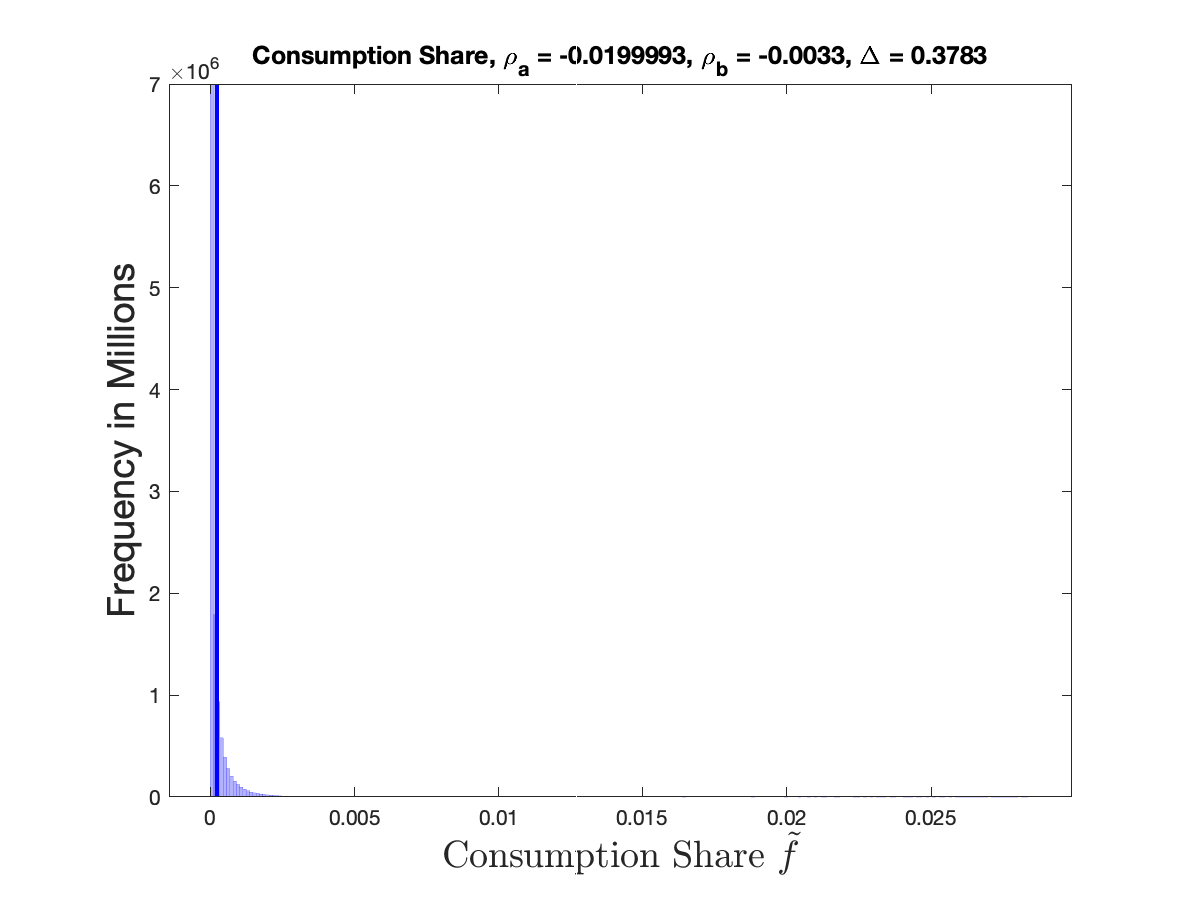
\includegraphics[width=.4\textwidth]{figures/IAFigCALn1.eps} &
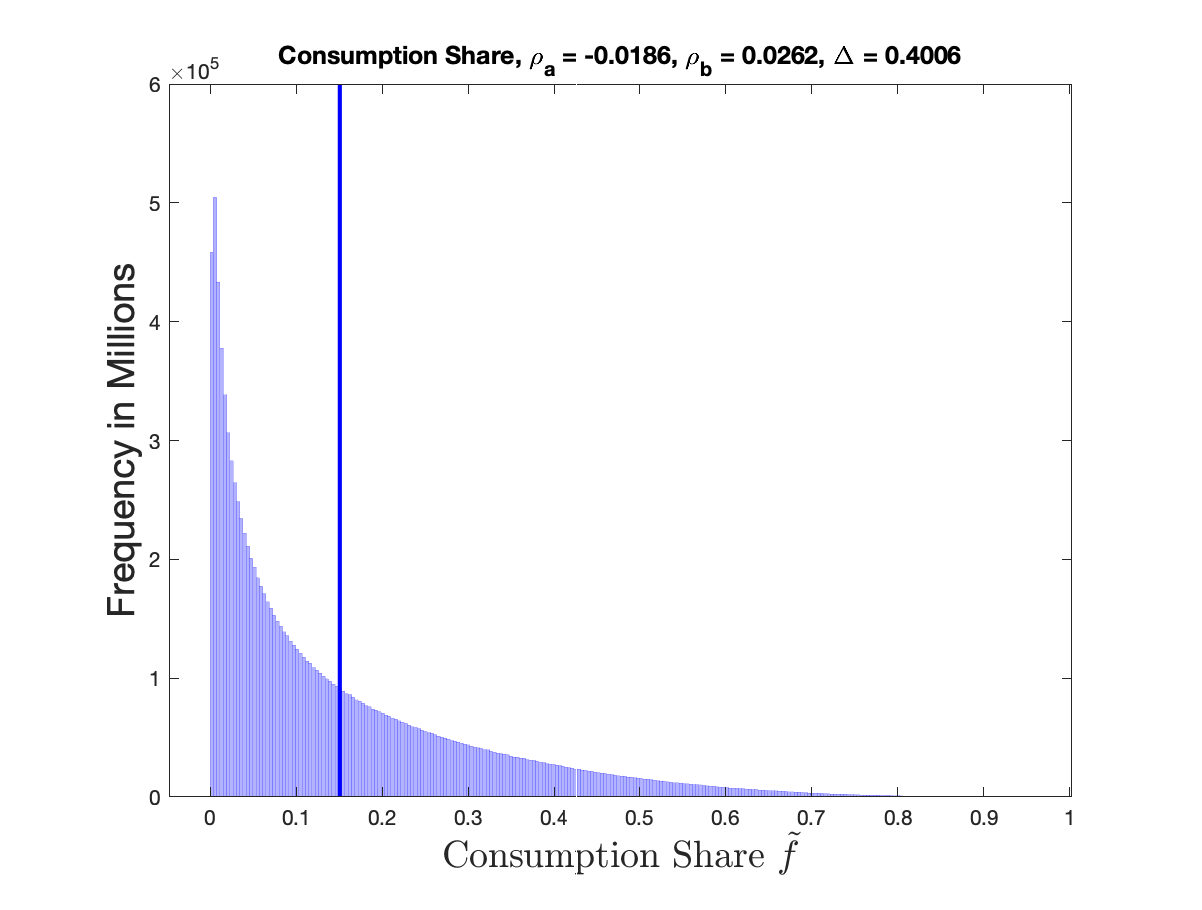
\includegraphics[width=.4\textwidth]{figures/IAFigCALn2.eps} \\
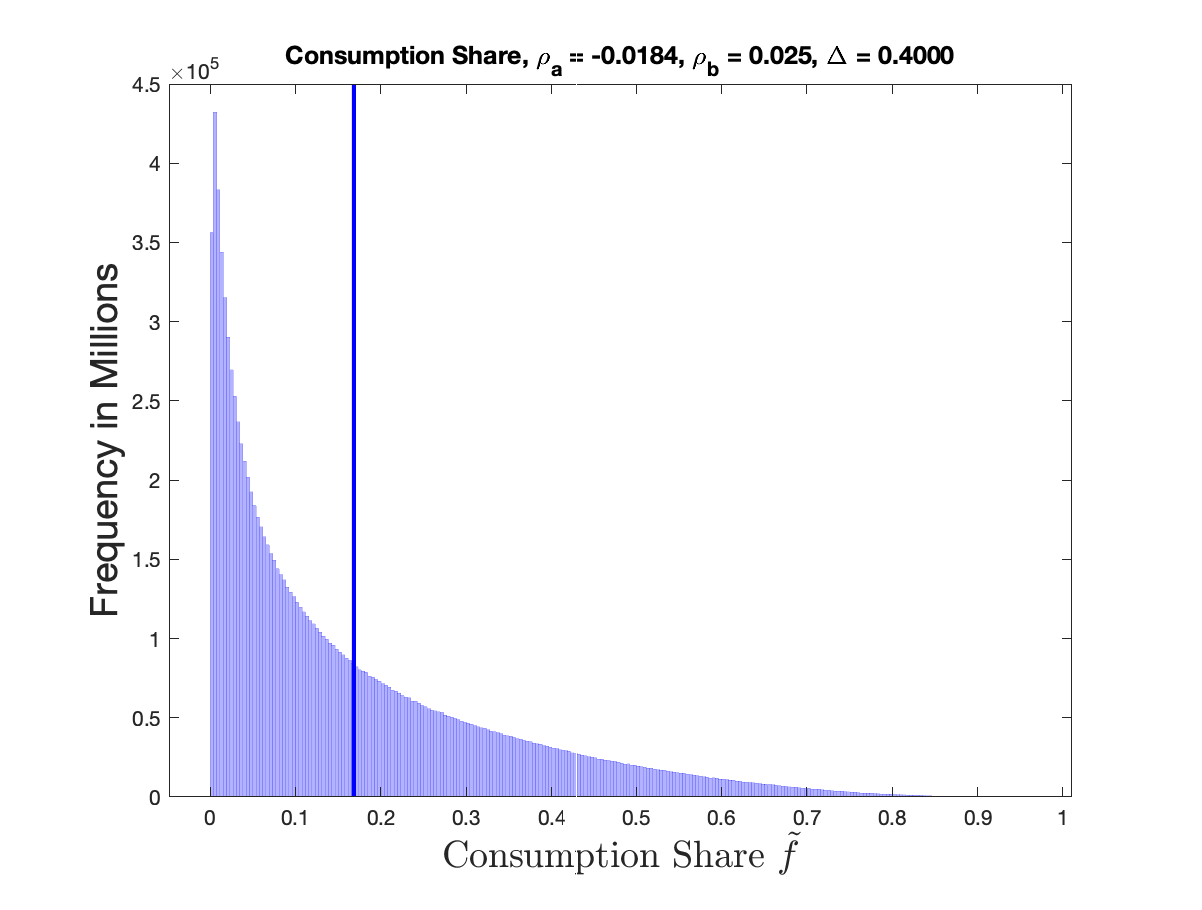
\includegraphics[width=.4\textwidth]{figures/IAFigCALn3.eps} &
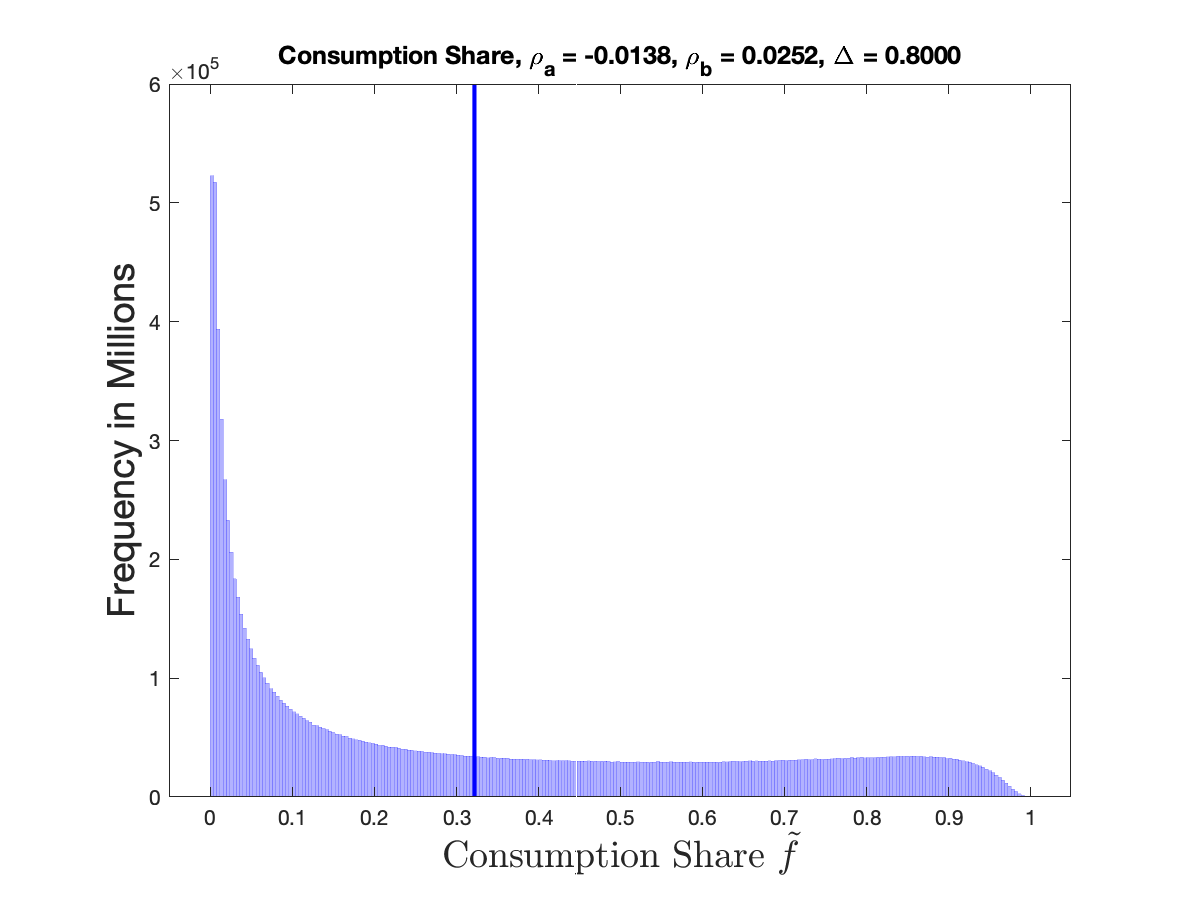
\includegraphics[width=.4\textwidth]{figures/IAFigCALn4.eps} \\
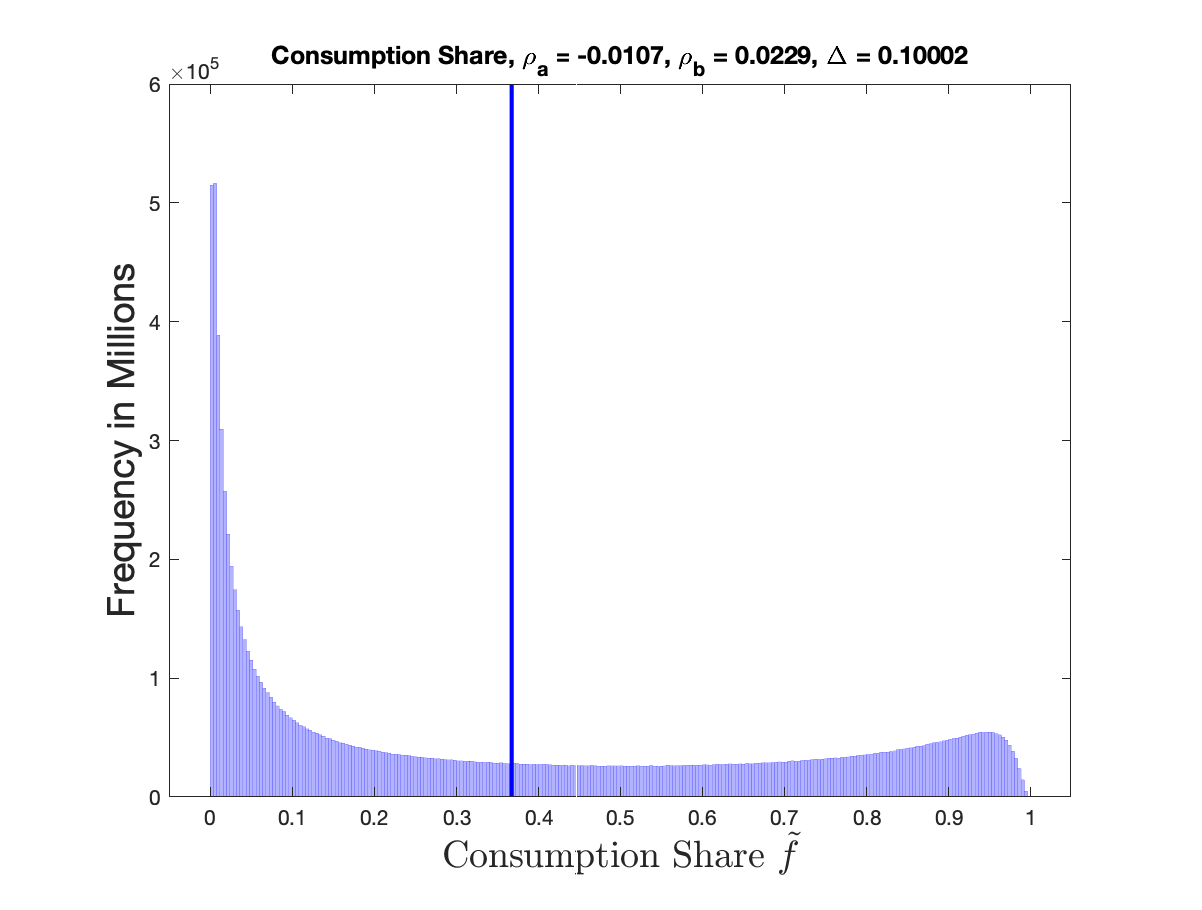
\includegraphics[width=.4\textwidth]{figures/IAFigCALn5.eps} &
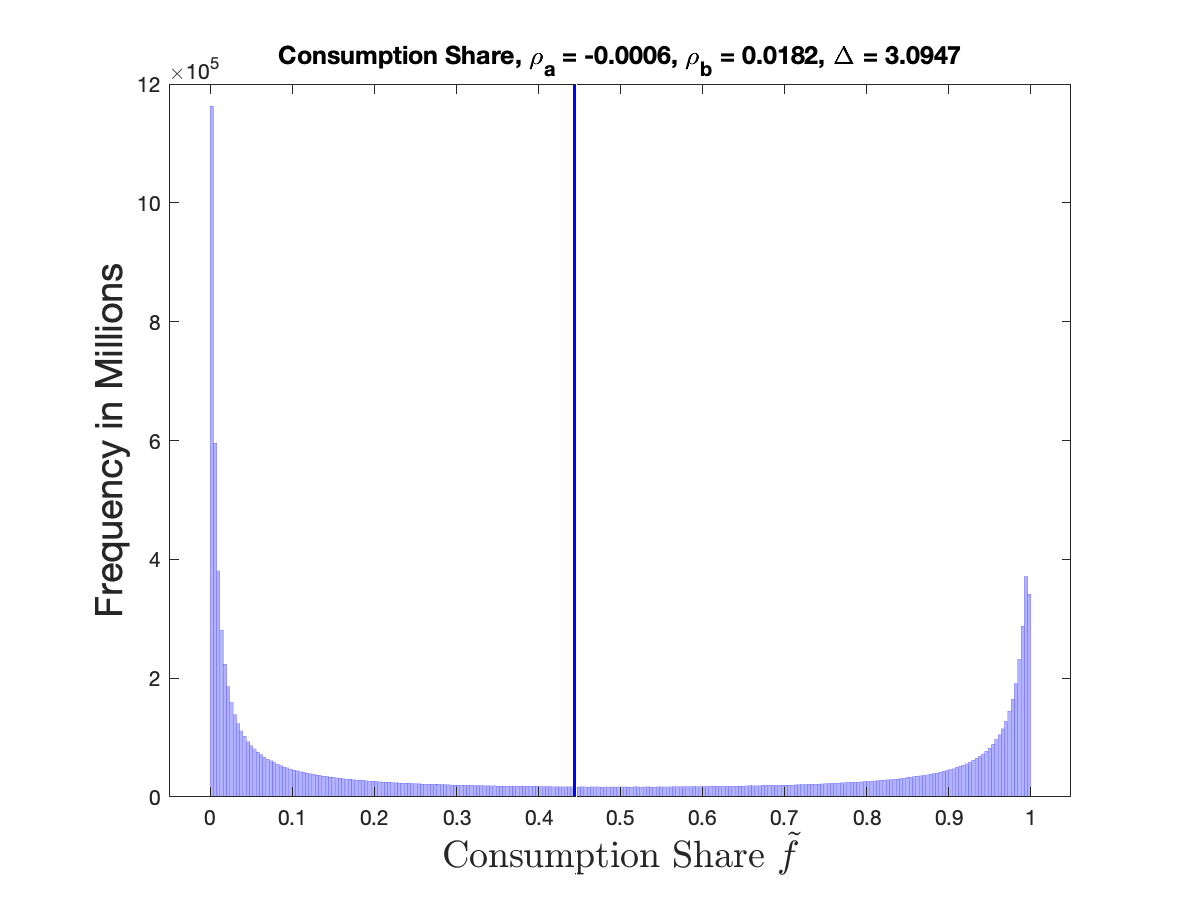
\includegraphics[width=.4\textwidth]{figures/IAFigCALn6.eps} 
\end{tabular}
\caption{\emph{Consumption share distribution for alternative set of parameters.}  \footnotesize{The graphs show the unconditional distribution of the consumption share of patient investors $\tilde{f}$ for very different set of parameters. The histograms are based one million years of monthly observations for each value of disagreement $\Delta$.}}\label{figIA:rev}
\end{figure}

\section{Reverse False Consensus Bias}\label{IArevbias}

We study how disagreement about the future prevalence of patient and impatient newborn investors---which leads to demand disagreement---affects asset price. Hence, we need to specify the beliefs of patient and impatient investors. We assumed that both patient and impatient investors overestimate the prevalence of their own type. This assumption serves as a reasonable starting point as it is consistent with a large psychology literature on the false consensus bias which is a cognitive bias whereby people tend to overestimate the extent to which their own opinions, beliefs, preferences, values, and habits are normal and typical of those of others.  %

Reversing the false consensus bias does not lead to a reversal of our main results. While the sign of the market price of demand risk flips when patient investors think they are underrepresented and thus short the consol (see Proposition 3), the exposure of the consol return to the demand shock also flips sign (see Proposition 6). Since the risk premium is determined by the product of these two terms, the overall risk premium remains unaffected (see Proposition 6). Hence, there are no qualitative changes to our results when the sign of the bias is reversed. This symmetry means that the key asset pricing implications are robust to the direction of the bias. 

However, there are minor quantitative differences in the moments of unconditional asset prices because the unconditional joint distribution of the two state variables depends on the sign of the bias. Specifically, with our preferred specification of the false consensus bias, a positive demand shock leads to more newborn impatient investors (higher $\alpha_t$) and an increase in their consumption share (higher $f_t$), amplifying price impact and demand for savings. With the reverse bias, a positive demand shock still increases the prevalence of newborn patient investors (higher $\alpha_t$) and raises the demand for savings, but now it lowers their consumption share (lower $f_t$). This subtle difference leads to slightly different unconditional asset pricing moments. We show unconditional moments of the consumption share, short rate, market price of demand shock risk, nominal bond yields, and nominal bond yield volatility in the tables below below.  For the false consensus bias with disagreement $\Delta = 0.8$, the mean and volatility of the consumption share are higher, the yields are slightly higher, and the yield volatilities are lower compared to reverse false consensus bias with the same amount of disagreement $\Delta = -0.8$.  




\begin{table}[h!]
\centering
\caption{\textbf{Unconditional moments of $f$, $r$, and $\theta$ with a false consensus bias:} This table presents the unconditional mean and volatility of the consumption share, the risk-free rate, and the market price of demand risk when there is a false consensus bias. These moments are derived from simulated unconditional distributions of $\tilde{\alpha}$ and $\tilde{f}$ across various demand disagreement levels ($\sigma_{\Delta}$), based on $500,000$ years of monthly model simulations.}
\begin{tabular}{|l|l|l|l|l|l|l|l|}
\hline
$\Delta$ & $\mathrm{E}[\tilde{f}]$ & $\mathrm{\sigma}[\tilde{f}]$ & $\mathrm{E}[\tilde{r}]$ & $\mathrm{\sigma}[\tilde{r}]$ 
& $\mathrm{E}[\tilde{\theta}_{\alpha}]$ & $\mathrm{\sigma}[\tilde{\theta}_{\alpha}]$ \\
\hline
0.0   & 0.3344 & 0.0992 & 0.0117 & 0.0052 & -    & -      \\
0.1   & 0.3334 & 0.1413 & 0.0128 & 0.0073 & 0.0167 & 0.0141 \\
0.2   & 0.3326 & 0.1863 & 0.0143 & 0.0133 & 0.0335 & 0.0373 \\
0.3   & 0.3185 & 0.2167 & 0.0162 & 0.0179 & 0.0544 & 0.0650 \\
0.4   & 0.3173 & 0.2447 & 0.0173 & 0.0213 & 0.0731 & 0.0979 \\
0.5   & 0.3077 & 0.2623 & 0.0184 & 0.0240 & 0.0961 & 0.1311 \\
0.6   & 0.2970 & 0.2747 & 0.0194 & 0.0260 & 0.1218 & 0.1648 \\
0.7   & 0.2946 & 0.2855 & 0.0197 & 0.0277 & 0.1437 & 0.1998 \\
0.8   & 0.2900 & 0.2940 & 0.0200 & 0.0292 & 0.1680 & 0.2352 \\
\hline
\end{tabular}
\end{table}
\begin{table}[h!]
\centering
\caption{\textbf{Unconditional moments of $f$, $r$, and $\theta$ with reverse false consensus bias:} This table presents the unconditional mean and volatility of the consumption share, the risk-free rate, and the market price of demand risk when there is a reverse false consensus bias. These moments are derived from simulated unconditional distributions of $\tilde{\alpha}$ and $\tilde{f}$ across various demand disagreement levels ($\sigma_{\Delta}$), based on $500,000$ years of monthly model simulations.}
\begin{tabular}{|l|l|l|l|l|l|l|l|}
\hline
$\Delta$ & $\mathrm{E}[\tilde{f}]$ & $\mathrm{\sigma}[\tilde{f}]$ & $\mathrm{E}[\tilde{r}]$ & $\mathrm{\sigma}[\tilde{r}]$ 
& $\mathrm{E}[\tilde{\theta}_{\alpha}]$ & $\mathrm{\sigma}[\tilde{\theta}_{\alpha}]$ \\
\hline
0.0    & 0.3344 & 0.0992 & 0.0117 & 0.0052 & -      & -      \\
-0.1   & 0.3186 & 0.0898 & 0.0124 & 0.0125 & -0.0181  & 0.0090 \\
-0.2   & 0.2956 & 0.1207 & 0.0140 & 0.0200 & -0.0409  & 0.0241 \\
-0.3   & 0.2774 & 0.1562 & 0.0155 & 0.0257 & -0.0668  & 0.0468 \\
-0.4   & 0.2664 & 0.1850 & 0.0164 & 0.0299 & -0.0935  & 0.0740 \\
-0.5   & 0.2611 & 0.2086 & 0.0170 & 0.0330 & -0.1195  & 0.1043 \\
-0.6   & 0.2582 & 0.2267 & 0.0172 & 0.0354 & -0.1451  & 0.1360 \\
-0.7   & 0.2611 & 0.2429 & 0.0164 & 0.0377 & -0.1672  & 0.1700 \\
-0.8   & 0.2597 & 0.2554 & 0.0168 & 0.0393 & -0.1923 & 0.2043 \\
\hline
\end{tabular}
\end{table}
\begin{table}[h!]
\centering
\caption{\textbf{Unconditional mean of yields with a false consensus bias:} This table presents the unconditional mean of yields with maturities ranging from one two ten years when there is a false consensus bias. These moments are derived from simulated unconditional distributions of $\tilde{\alpha}$ and $\tilde{f}$ across various demand disagreement levels ($\sigma_{\Delta}$), based on $500,000$ years of monthly model simulations.}
\begin{tabular}{c|ccccccc}
\hline
$\Delta$ & Mean y1 & Mean y2 & Mean y3 & Mean y4 & Mean y5 & Mean y7 & Mean y10 \\
\hline
0.0 & 0.0117 & 0.0117 & 0.0117 & 0.0117 & 0.0117 & 0.0117 & 0.0117 \\
0.1 & 0.0128 & 0.0128 & 0.0128 & 0.0128 & 0.0128 & 0.0128 & 0.0128 \\
0.2 & 0.0143 & 0.0143 & 0.0144 & 0.0144 & 0.0145 & 0.0145 & 0.0146 \\
0.3 & 0.0163 & 0.0164 & 0.0165 & 0.0166 & 0.0167 & 0.0168 & 0.0170 \\
0.4 & 0.0174 & 0.0176 & 0.0177 & 0.0178 & 0.0179 & 0.0181 & 0.0184 \\
0.5 & 0.0186 & 0.0188 & 0.0190 & 0.0191 & 0.0193 & 0.0196 & 0.0199 \\
0.6 & 0.0196 & 0.0199 & 0.0201 & 0.0203 & 0.0205 & 0.0208 & 0.0212 \\
0.7 & 0.0200 & 0.0203 & 0.0206 & 0.0208 & 0.0210 & 0.0214 & 0.0219 \\
0.8 & 0.0204 & 0.0207 & 0.0210 & 0.0213 & 0.0216 & 0.0220 & 0.0225 \\
\hline
\end{tabular}
\end{table}

\begin{table}[h!]
\centering
\caption{\textbf{Unconditional mean of yields with a reverse false consensus bias:} This table presents the unconditional mean of yields with maturities ranging from one two ten years when there is a reverse false consensus bias. These moments are derived from simulated unconditional distributions of $\tilde{\alpha}$ and $\tilde{f}$ across various demand disagreement levels ($\sigma_{\Delta}$), based on $500,000$ years of monthly model simulations.}
\begin{tabular}{c|ccccccc}
\hline
$\Delta$ & Mean y1 & Mean y2 & Mean y3 & Mean y4 & Mean y5 & Mean y7 & Mean y10 \\
\hline
0.0  & 0.0117 & 0.0117 & 0.0117 & 0.0117 & 0.0117 & 0.0117 & 0.0117 \\
-0.1 & 0.0124 & 0.0125 & 0.0125 & 0.0125 & 0.0125 & 0.0125 & 0.0125 \\
-0.2 & 0.0141 & 0.0142 & 0.0143 & 0.0144 & 0.0144 & 0.0145 & 0.0145 \\
-0.3 & 0.0157 & 0.0158 & 0.0160 & 0.0161 & 0.0162 & 0.0164 & 0.0165 \\
-0.4 & 0.0167 & 0.0170 & 0.0172 & 0.0173 & 0.0175 & 0.0177 & 0.0180 \\
-0.5 & 0.0173 & 0.0176 & 0.0179 & 0.0181 & 0.0183 & 0.0186 & 0.0190 \\
-0.6 & 0.0176 & 0.0180 & 0.0183 & 0.0186 & 0.0188 & 0.0192 & 0.0196 \\
-0.7 & 0.0169 & 0.0173 & 0.0177 & 0.0180 & 0.0183 & 0.0188 & 0.0193 \\
-0.8 & 0.0173 & 0.0178 & 0.0181 & 0.0185 & 0.0188 & 0.0193 & 0.0199 \\
\hline
\end{tabular}
\end{table}

\begin{table}[h!]
\centering
\caption{\textbf{Unconditional volatility of yields with a false consensus bias:} This table presents the unconditional volatility of yields with maturities ranging from one two ten years when there is a false consensus bias. These moments are derived from simulated unconditional distributions of $\tilde{\alpha}$ and $\tilde{f}$ across various demand disagreement levels ($\sigma_{\Delta}$), based on $500,000$ years of monthly model simulations.}
\begin{tabular}{c|ccccccc}
\hline
$\Delta$ & Std Y1 & Std Y2 & Std Y3 & Std Y4 & Std Y5 & Std Y7 & Std Y10 \\
\hline
0.0 & 0.0051 & 0.0050 & 0.0049 & 0.0048 & 0.0047 & 0.0045 & 0.0043 \\
0.1 & 0.0073 & 0.0073 & 0.0072 & 0.0072 & 0.0072 & 0.0071 & 0.0070 \\
0.2 & 0.0132 & 0.0130 & 0.0129 & 0.0127 & 0.0126 & 0.0123 & 0.0119 \\
0.3 & 0.0176 & 0.0174 & 0.0171 & 0.0169 & 0.0166 & 0.0162 & 0.0156 \\
0.4 & 0.0209 & 0.0206 & 0.0202 & 0.0199 & 0.0196 & 0.0190 & 0.0182 \\
0.5 & 0.0235 & 0.0230 & 0.0226 & 0.0222 & 0.0218 & 0.0211 & 0.0201 \\
0.6 & 0.0255 & 0.0249 & 0.0244 & 0.0239 & 0.0234 & 0.0226 & 0.0215 \\
0.7 & 0.0271 & 0.0264 & 0.0258 & 0.0252 & 0.0247 & 0.0237 & 0.0225 \\
0.8 & 0.0285 & 0.0277 & 0.0270 & 0.0264 & 0.0258 & 0.0247 & 0.0234 \\
\hline
\end{tabular}
\end{table}

\begin{table}[h!]
\centering
\caption{\textbf{Unconditional volatility of yields with a false consensus bias:} This table presents the unconditional volatility of yields with maturities ranging from one two ten years when there is a reverse false consensus bias. These moments are derived from simulated unconditional distributions of $\tilde{\alpha}$ and $\tilde{f}$ across various demand disagreement levels ($\sigma_{\Delta}$), based on $500,000$ years of monthly model simulations.}
\begin{tabular}{c|ccccccc}
\hline
$\Delta$ & Std Y1 & Std Y2 & Std Y3 & Std Y4 & Std Y5 & Std Y7 & Std Y10 \\
\hline
0.0   & 0.0051 & 0.0050 & 0.0049 & 0.0048 & 0.0047 & 0.0045 & 0.0043 \\
-0.1  & 0.0122 & 0.0119 & 0.0116 & 0.0113 & 0.0110 & 0.0104 & 0.0097 \\
-0.2  & 0.0195 & 0.0190 & 0.0185 & 0.0181 & 0.0177 & 0.0169 & 0.0158 \\
-0.3  & 0.0250 & 0.0243 & 0.0237 & 0.0232 & 0.0227 & 0.0217 & 0.0204 \\
-0.4  & 0.0290 & 0.0283 & 0.0275 & 0.0269 & 0.0263 & 0.0252 & 0.0237 \\
-0.5  & 0.0321 & 0.0312 & 0.0304 & 0.0297 & 0.0290 & 0.0278 & 0.0262 \\
-0.6  & 0.0344 & 0.0334 & 0.0325 & 0.0317 & 0.0310 & 0.0297 & 0.0280 \\
-0.7  & 0.0365 & 0.0355 & 0.0345 & 0.0336 & 0.0328 & 0.0314 & 0.0297 \\
-0.8  & 0.0380 & 0.0369 & 0.0359 & 0.0350 & 0.0342 & 0.0327 & 0.0309 \\
\hline
\end{tabular}
\end{table} 




\section{General Disagreement}

In this section we provide some details on general disagreement as discussed in Section IV.A in the paper. Specifically, as in the paper let $\Delta^i_{s,t}$ be the estimation error  at time $t$ of an agent of type $i$ born at time $s$. As before, the agents' perceived shocks are related to the true shock in the following way:
\begin{equation}
	dz^i_{s,t} = dz_{\alpha,t} - \Delta^i_{s,t}dt.
\end{equation}
The likelihood ratio, $\eta^i_{s,t}$, which represents the change of measure between the belief of agent $i$ born at time $s$ at time $t$ and the data generating probability measure has the dynamics
\begin{equation}
	d\eta^i_{s,t} = \Delta^i_{s,t} \eta^i_{s,t}dz_{\alpha,t}.
\end{equation}
We now provide details of Proposition 10 in the paper. First, from the FOC we have that:
\begin{equation}\label{IAoptimalconsumption}
	 c^i_{s,t} =c^i_{s,s} e^{-\rho_i \left(t-s\right)}\frac{\eta^i_{s,t}}{\eta^i_{s,s}} \frac{\xi_{s}}{\xi_{t}}
\end{equation}
Inserting optimal consumption given in Equation (\ref{IAoptimalconsumption}) into the market clearing condition we get
\begin{eqnarray}
	Y_t &=& \int_{-\infty}^{t} \nu e^{-\nu\left(t-s\right)}\left(\alpha_s c^a_{s,s} e^{-\rho_a \left(t-s\right)}\frac{\eta^a_{s,t}}{\eta^a_{s,s}} \frac{\xi_{s}}{\xi_{t}} + \left(1-\alpha_s\right)c^b_{s,s} e^{-\rho_b \left(t-s\right)}\frac{\eta^b_{s,t}}{\eta^b_{s,s}} \frac{\xi_{s}}{\xi_{t}}\right)ds \nonumber \\
	\xi_t Y_t &=& \int_{-\infty}^{t} \nu e^{-\nu\left(t-s\right)}\left(\alpha_s \beta^a_{s}e^{-\rho_a \left(t-s\right)}\frac{\eta^a_{s,t}}{\eta^a_{s,s}} + \left(1-\alpha_s\right)\beta^b_s e^{-\rho_b \left(t-s\right)}\frac{\eta^b_{s,t}}{\eta^b_{s,s}}\right)\xi_s Y_s ds \nonumber \\
		X_t &=& \int_{-\infty}^{t} \nu e^{-\nu\left(t-s\right)}\left(\alpha_s \beta^a_{s}e^{-\rho_a \left(t-s\right)}\frac{\eta^a_{s,t}}{\eta^a_{s,s}} + \left(1-\alpha_s\right)\beta^b_s e^{-\rho_b \left(t-s\right)}\frac{\eta^b_{s,t}}{\eta^b_{s,s}}\right)X_s ds, 
\end{eqnarray}
where $X_t = \xi_t Y_t$ implying $\xi_t = \frac{X_t}{Y_t}$. As before, we get for the consumption share of all patient investors:  $f_t = \int_{-\infty}^{t} \nu e^{-\nu\left(t-s\right)}\left(\alpha_s \beta^a_{s}e^{-\rho_a \left(t-s\right)}\frac{\eta^a_{s,t}}{\eta^a_{s,s}}\right)\frac{X_s}{X_t} ds$. An application of Ito's lemma 
gives
\begin{eqnarray}
	dX_t &=& X_t\left( \nu\left(\alpha_t \beta^a_t + \left(1-\alpha_t\right)\beta^b_t - 1\right)  - \rho_a f_t - \rho_b \left(1-f_t\right)\right) dt  \nonumber \\
	&&+ X_t\left(\bar{\Delta}^{a}_t f_t + \bar{\Delta}^b_t \left(1-f_t\right)\right)dZ_{\alpha,t},
\end{eqnarray}
where 
\begin{equation}
	\bar{\Delta}^i_t = \int_{-\infty}^{t} \bar{f}^i_{s,t} \Delta^i_{s,t}ds,  \qquad i=a,b,
\end{equation}
where  the within group consumption share densities are
\begin{eqnarray}
	\bar{f}^a_{s,t} &=&\left(\frac{1}{f_t}\right)\nu e^{-\left(\rho^a+\nu\right)\left(t-s\right)} \alpha_s \beta^a_{s}\left(\frac{\eta^a_{s,t}}{\eta^a_{s,s}}\right)\left(\frac{Y_s}{Y_t}\right)\left(\frac{\xi_s}{\xi_t}\right)\\
	\bar{f}^b_{s,t} &=& \left(\frac{1}{1-f_t}\right)\nu e^{-\left(\rho^b+\nu\right)\left(t-s\right)} \left(1-\alpha_s\right) \beta^b_{s}\left(\frac{\eta^b_{s,t}}{\eta^b_{s,s}}\right)\left(\frac{Y_s}{Y_t}\right)\left(\frac{\xi_s}{\xi_t}\right).
\end{eqnarray}
An application of Ito's lemma to $\xi_t = \frac{X_t}{Y_t}$ yields the following. 

\begin{prop}\label{SDFgeneralDIS}
The real short rate, $r_t$, and the market price of supply shocks, $\theta_{Y,t}$, take the same form as before and are given Proposition \ref{prop_rtandtheta}. The market price of demand shocks is 
\begin{equation}
\theta_{\alpha,t} %= - \bar{\Delta}_t  
= -\left(f_t \bar{\Delta}^a_t + \left(1-f_t\right)\bar{\Delta}^b_t\right), 
\end{equation}
where $f_t$ is the fraction of output consumed by all agents of type $a$. The within type $i$ consumption share weighted average estimation error is 
\begin{equation}
	\bar{\Delta}^i_t = \int_{-\infty}^{t} \bar{f}^i_{s,t} \Delta^i_{s,t}ds,  \qquad i=a,b,
\end{equation}
where  the within group consumption share densities are
\begin{eqnarray}
	\bar{f}^a_{s,t} &=&\left(\frac{1}{f_t}\right)\nu e^{-\left(\rho^a+\nu\right)\left(t-s\right)} \alpha_s \beta^a_{s}\left(\frac{\eta^a_{s,t}}{\eta^a_{s,s}}\right)\left(\frac{Y_s}{Y_t}\right)\left(\frac{\xi_s}{\xi_t}\right)\\
	\bar{f}^b_{s,t} &=& \left(\frac{1}{1-f_t}\right)\nu e^{-\left(\rho^b+\nu\right)\left(t-s\right)} \left(1-\alpha_s\right) \beta^b_{s}\left(\frac{\eta^b_{s,t}}{\eta^b_{s,s}}\right)\left(\frac{Y_s}{Y_t}\right)\left(\frac{\xi_s}{\xi_t}\right)
\end{eqnarray}
with $\beta^i_t = \left(\rho^i + \nu\right)\phi_t$ and the wealth-consumption ratio, $\phi_t$, as before. The stock price- and console dynamics are the same as in the baseline model where the constant disagreement, $\Delta$, is replaced with the stochastic disagreement $\Delta_t= \bar{\Delta}^a_t - \bar{\Delta}^b_t$. 
\end{prop}

The consumption share, $f_t$, is still an endogenous state variable but the within group consumption share weighted estimation errors replace the constant estimation errors from the previous section. Importantly, the risk-free rate and market prices of risk take similar forms as in the case without learning. Although it is sufficient to know $\alpha_t$, $f_t$ and $\bar{\Delta}_t$ to characterize the equilibrium at any point in time, the dynamics of $f_t$ and $\bar{\Delta}_t$ do not form a Markov system, but require the knowledge of every agent's belief. We now consider a special case where agents learn from their own experience. 

\subsection{Demand Disagreement with Learning from Experience}

In the baseline, model we made two assumptions about preferences and beliefs. First, there is a strong link between preferences and beliefs as agents disagree across but not within preference types. Second, agents do not learn. In this section, we relax both of these assumptions by allowing agents to learn from their own experience as in \citeasnoun{EGH18}. 

We assume that an agent of type $i$ born at time $s$ has a normally distributed prior about the long-run mean of $l_t$, with mean $\bar{l}^i$ and variance $V$. Hence, everyone has the same prior variance, $V$, but patient and impatient agents might have different prior means, $\bar{l}^i$. The next proposition characterizes the time-t estimation error of an agent born at time $s$.
\begin{prop}\label{LearningEstimationError}
The time-$t$ estimation error of an agent of type $i=a,b$ born at time $s$ is 
\begin{equation}
	 \Delta^i_{s,t} = \frac{\sigma_{A}^2}{\sigma_{A}^2 + V\left(t-s\right)}\Delta^i_{s,s} + \frac{V}{\sigma_{A}^2 + V\left(t-s\right)}\left(Z_{\alpha,t}-Z_{\alpha,s}\right),
\end{equation}
where $\sigma_{A} = \frac{\sigma_l}{\kappa}$ and $\Delta^i_{s,s} = \frac{\bar{l}^i-\bar{l}}{\sigma_{A}}$. Moreover, we have that $\lim_{t\to\infty} \Delta^i_{s,t} =0$. Initial disagreement is  $\Delta = \Delta_{s,s}  = \Delta^a_{s,s}-\Delta^b_{s,s}$.
\end{prop} 
From Proposition \ref{LearningEstimationError}, we see that agents eventually learn the true long-run mean. However, this will typically take a long time, and therefore agents keep making mistakes for many years. Moreover, young agents update their beliefs more aggressively than older agents. To examine the effects of learning, we consider three different values of initial disagreement $\Delta = \left(0,0.4,0.8\right)$. If the common prior variance, $V$, is zero, then agents do not learn and we are back to the dogmatic beliefs case. However, once $V$ is positive, agents learn from their own experience and therefore different cohorts disagree, even without any initial disagreement $\Delta$.  

How does learning from experience affect the consumption share of patient and impatient investors? In contrast to the baseline model, investors learn over their lifetime and, thus, their beliefs are more accurate when they are older. Hence, more experienced investors are expected to gain wealth from less experienced investors. While this is true for both patient and impatient investors, the speculative profits are expected to be higher for patient than for impatient investors because they save more over time and therefore they are wealthier when their beliefs are more accurate.  The left graph of Figure \ref{CshareandDislearning} confirms this intuition. Specifically, it shows that even without any initial disagreement (black solid line) the unconditional mean of the consumption share, $\tilde{f}$, is increasing with the prior variance except for an initial drop that is due to the fact that everybody is born with the true prior.  Similarly, the average consumption share is increasing in the prior variance $V$ if we allow for initial disagreement as the blue dashed circle line and the red chain-dotted crossed line in the left graph in Figure \ref{CshareandDislearning} show. In contrast to the slight initial drop of the average consumption share when everybody starts with the correct prior, there is a stark initial increase of the average consumption share because investors initially disagree and, thus, have incorrect initial beliefs. 
  

\begin{figure}[htbp] 
\centering
\vspace{0.1in}
\begin{tabular}{ccc}
\includegraphics[width=.3\textwidth]{figures/FigLearning_f_v1.eps} &
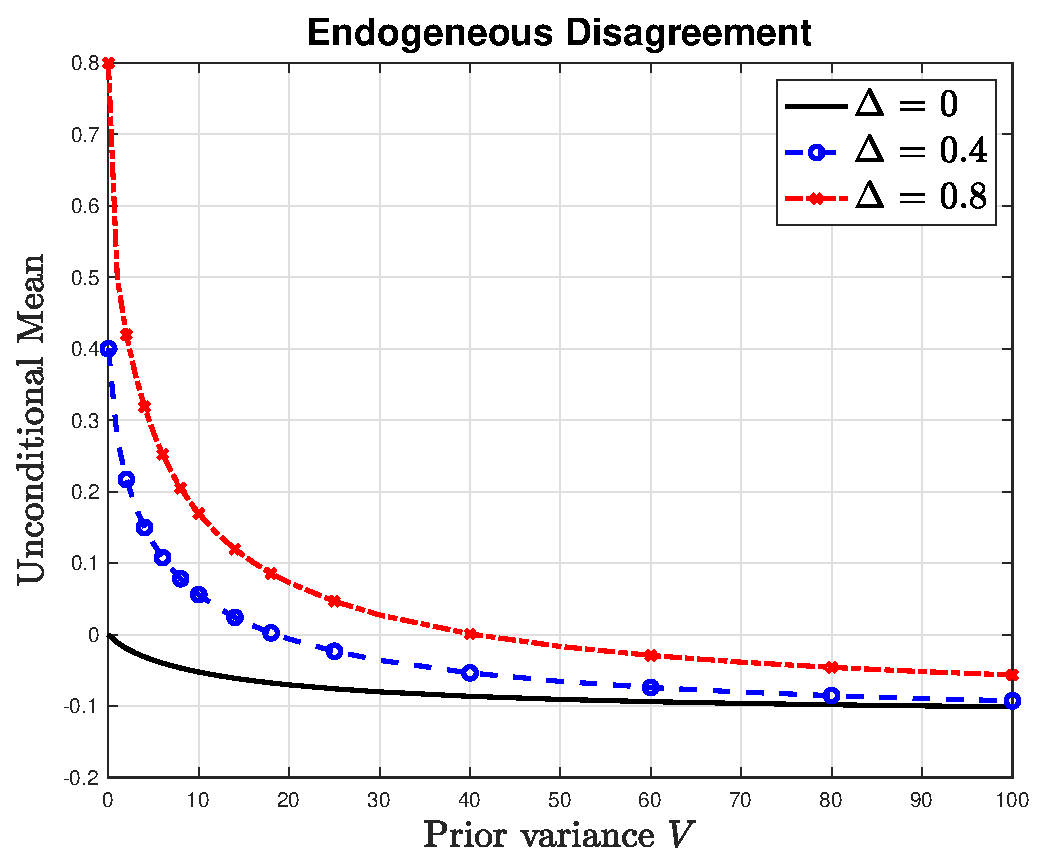
\includegraphics[width=.3\textwidth]{figures/FigLearning_DeltaM_v1.eps}
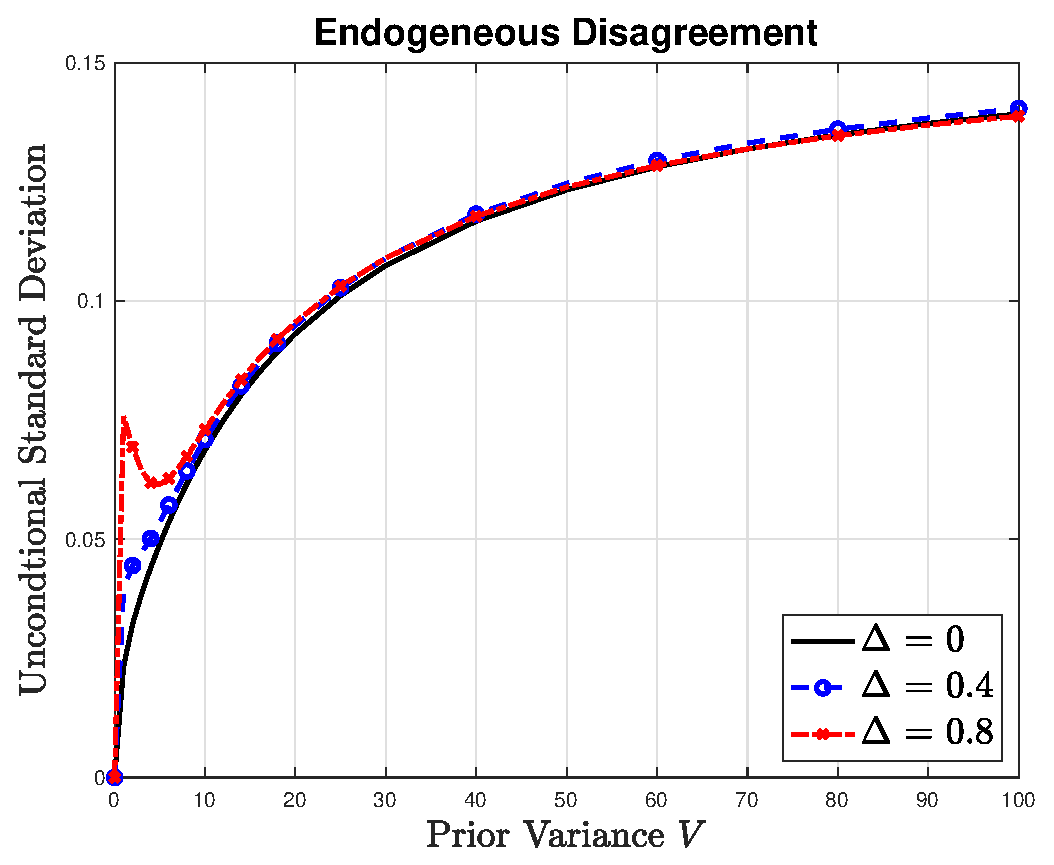
\includegraphics[width=.3\textwidth]{figures/FigLearning_DeltaSTD_v1.eps}
\end{tabular}
\caption{\emph{Unconditional moments of the consumption share and disagreement.} \footnotesize{This figure shows the unconditional mean of the consumption share (left), the unconditional mean of disagreement (middle) and the unconditional standard deviation of disagreement (right) as a function of the prior variance $V$ for different initial disagreement $\Delta$. All other parameters are as in the baseline calibration. The summary statistics are based on one million years of monthly observations for each prior variance value $V$.}} \label{CshareandDislearning} %We keep track of 12000 cohorts.}} \label{CshareandDislearning}
\end{figure}
 
The middle and right graph of Figure \ref{CshareandDislearning} show the unconditional mean and volatility of disagreement between patient and impatient investors $\Delta_t$, respectively. % given in Proposition \ref{LearningEstimationError}. 
As expected, this disagreement converges towards zero when $\Delta \neq 0$. However, this average is not zero even when all agents are born with the true prior (black solid line) because there is a correlation between the fraction of patient newborns $\alpha_t$ and disagreement $\Delta_t$. Importantly, the right plot shows that the standard deviation is increasing even for the case with no initial disagreement. This implies that ``typically'' there is more disagreement when the prior variance, $V$, is high even when the two groups start we the same beliefs. Hence, the model with learning from experience endogenously creates disagreement between the two groups of investors and as we show below implies similar asset pricing implications as the case without learning.  


Figure \ref{APlearningFIG} shows the average risk free rate (left plot), the standard deviation of the market return (middle plot) and the risk premium on the market (right plot) as we vary the prior variance $V$ for initial disagreement $\Delta=0, 0.4, 0.8$. As the prior variance increases, initial disagreement has less impact. If there is no initial disagreement ($\Delta=0$), then the standard deviation and risk premium are increasing in $V$ which implies more disagreement and so is similar to the case without learning. In contrast, the risk-free rate is decreasing with disagreement measured by V because the average consumption share of patient investors increases. 

\begin{figure}[htbp] 
\centering
\vspace{0.1in}
\begin{tabular}{ccc}
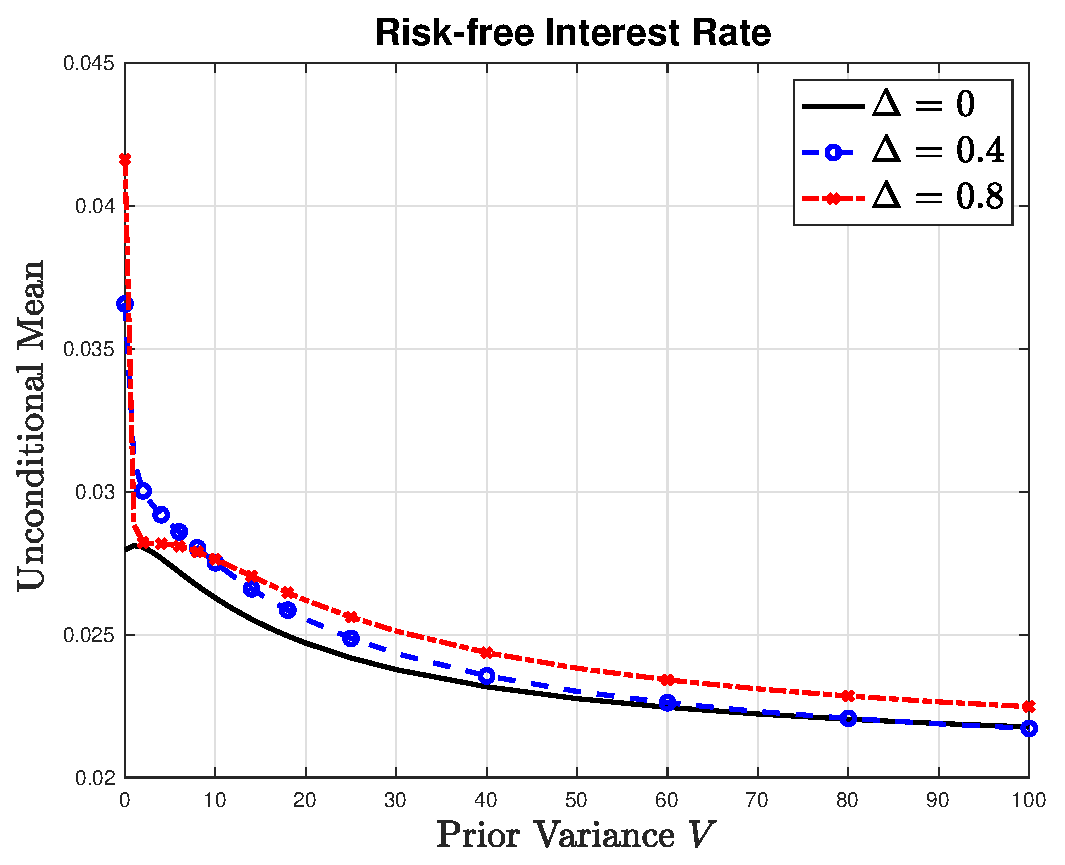
\includegraphics[width=.3\textwidth]{figures/Fig_learning_r_v1.eps} &
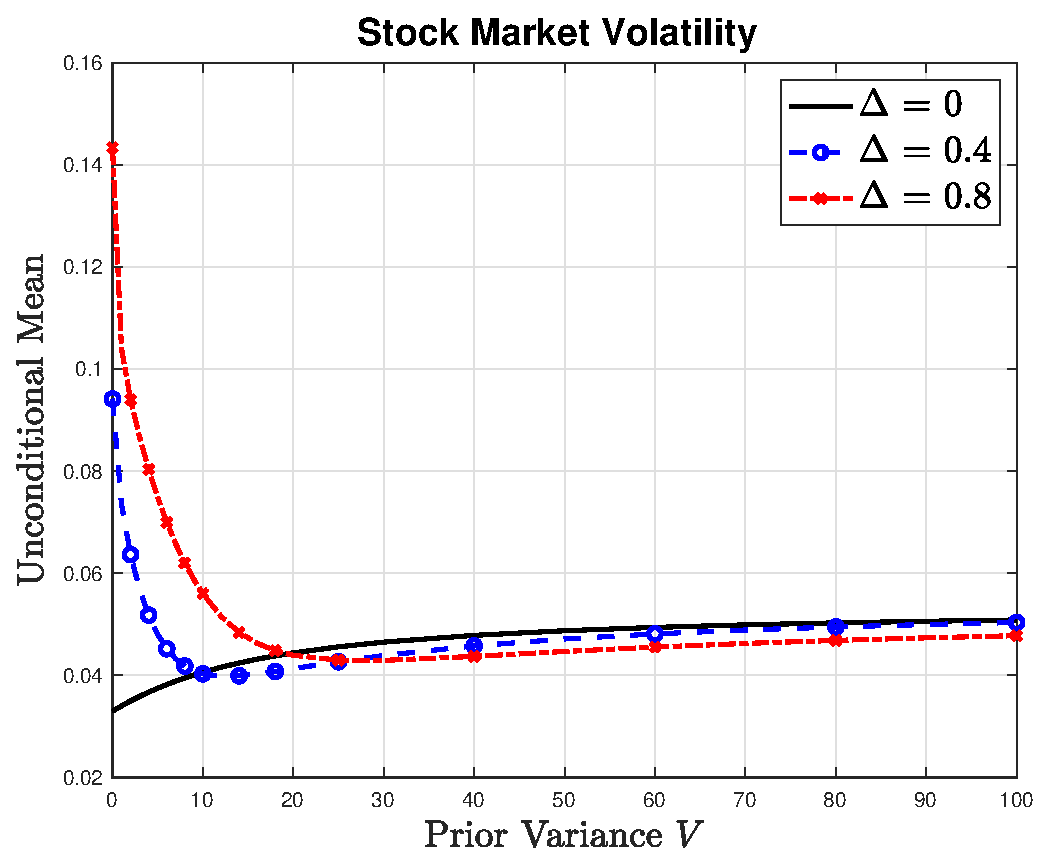
\includegraphics[width=.3\textwidth]{figures/Fig_learning_StdevRM_v1.eps}
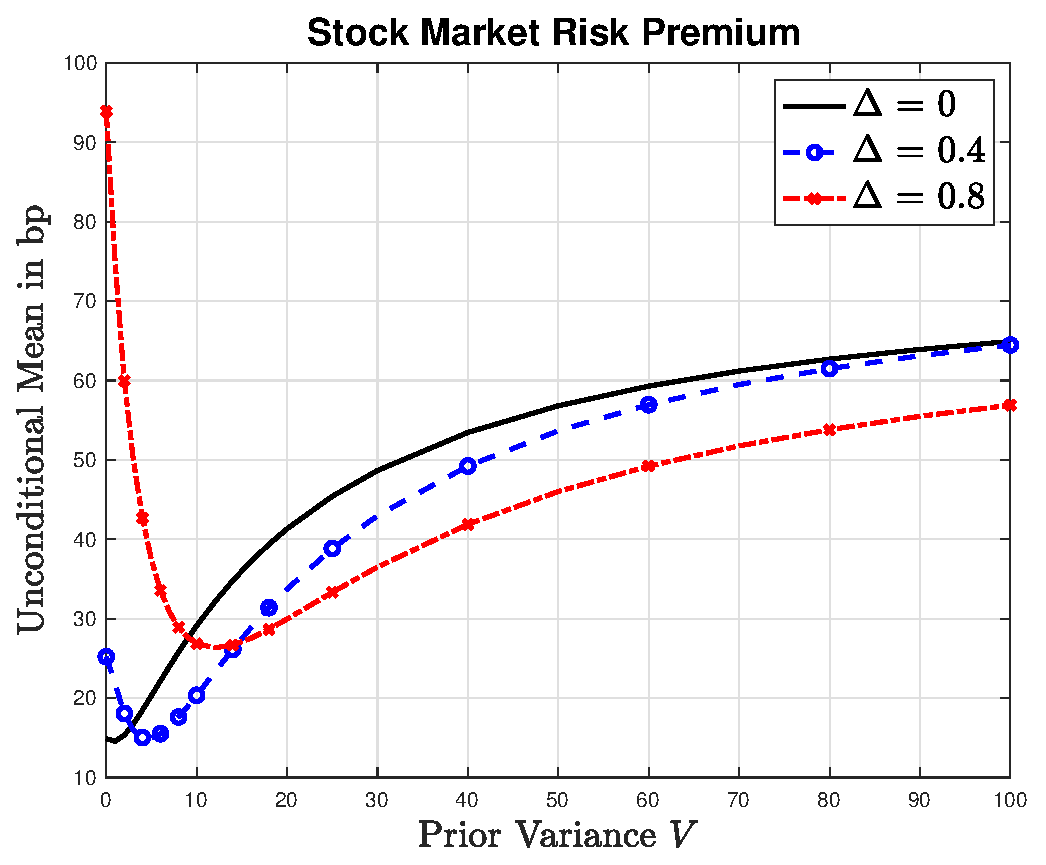
\includegraphics[width=.3\textwidth]{figures/Fig_learning_RiskP_v1.eps}
\end{tabular}
\caption{\emph{Asset pricing with learning from experience.} \footnotesize{The figure shows the unconditional mean of the risk free rate (left plot), stock market volatility (middle plot), and stock market risk premium (right plot) as a function of the prior variance (disagreement) for different initial disagreement $\Delta$ set to $0$, $0.4$ and $0.8$.  All other parameters are as in the baseline calibration. The summary statistics are based on one million years of monthly observations for each prior variance value $V$.}} \label{APlearningFIG} %We keep track of 12000 cohorts.
\end{figure}


\section{Production Economy}

In this section, we provide some more details on the production economy studied in Section IV.B in the paper. Agents are endowed with capital instead of a Lucas tree. Capital is traded and agents agree on its price. The capital of agents who die is reallocated to the newborn agents. Investors face dynamically complete security markets as in the case of our exchange economy. The dynamics of capital are
\begin{equation}
	dK_t = \left(\psi \left(\iota_t\right) + \mu_K-\delta\right)K_t \:  dt + \sigma_K K_t \: dZ_{K,t}.
\end{equation}
Investments are subject to an adjustment costs represented by the function, $\psi \left(\iota\right) = \frac{log\left(\kappa \iota + 1\right)}{\kappa}$, where $\iota_t$ is the investment rate per unit of capital and $\kappa$ is the investment cost parameter. The second component of the expected growth rate in capital is, $\mu_K-\delta$, where $\mu_K$ represents productivity improvements and $\delta$ is depreciation. One unit of capital produces $a$ units of the consumption good and thus output is $Y_t = a K_t$.\footnote{One can show that all agents will make the same choice, and therefore we do not model the investment choice of each individual agent but instead consider the representative firm.} The resource constraint is $Y_t = C_t + I_t$ where aggregate investment is $I_t=\iota_t K_t$. Let $Q_t$ denote the price of capital which is determined in equilibrium. We posit that the dynamics of $Q_t$ are
\begin{equation}
	dQ_t = Q_t\left(\mu_{Q,t} dt + \sigma^{K}_{Q,t} dZ_{K,t} + \sigma^{\alpha}_{Q,t} dZ_{\alpha,t} \right),
\end{equation}
where the drift, $\mu_{Q,t}$, the supply shock exposure, $\sigma^{K}_{Q,t}$, and the demand shock exposure, $\sigma^{\alpha}_{Q,t}$ will be determined in equilibrium. Given the optimal investment rate, $\iota_t$, the firm pays out $D_t = \left(a-\iota_t\right)K_t$ in dividends and by market clearing we have that $C_t = D_t$. Moreover, the total value of the firm is $S_t = Q_t K_t$ and thus the total return on the stock market is
{\small
\begin{align}
	dR_t &=  \frac{D_t}{S_t}dt + \frac{dS_t}{S_t} = \frac{D_t}{S_t}dt + \frac{dK_t}{K_t}  + \frac{dQ_t}{Q_t} + \frac{dK_t}{K_t} \frac{dQ_t}{Q_t} \nonumber \\
	        &=  \left(\frac{a-\iota_t}{Q_t} + \psi   \left(\iota_t\right)  + \mu_K-\delta + \mu_{Q,t} + \sigma_K \sigma^{K}_{Q,t}\right)dt  
	         + \left(\sigma_K+ \sigma^{K}_{Q,t}\right)dZ_{Y,t} + \sigma^{\alpha}_{Q,t}dZ_{\alpha,t}.
\end{align}
}
To obtain the optimal investment rate, we maximize the value of the firm which is equivalent to 
\begin{equation}\label{IAprodOptInv}
	\underset{\{\iota_t \}}{\max} \quad E [ dR_t].
\end{equation}
state by state. The FOC of the firm's maximization problem in Equation (\ref{IAprodOptInv}) is $\frac{1}{Q_t} = \psi' \left(\iota_t\right)$. Using the expression for the adjustment cost function and solving it for the investment rate, $\iota_t$, we get
\begin{equation}\label{optinv}
	\iota_t = \frac{Q_t - 1}{\kappa}.
\end{equation}
Total wealth in the economy is $S_t = Q_t K_t$ and so the following holds true
\begin{equation}\label{ClearingW}
 \begin{split}	
 	S_t &= Q_t K_t = \int_{-\infty}^t \nu e^{-\nu\left(t-s\right)}\left(\alpha_{s,t}W^a_{s,t} + \left(1-\alpha_{s,t}\right)W^b_{s,t}\right)ds  \\
	&=z  \int_{-\infty}^t \nu e^{-\nu\left(t-s\right)}\left(\alpha_{s,t}\frac{C^a_{s,t}}{\rho_a+\nu} 
	+ \left(1-\alpha_{s,t}\right)\frac{C^b_{s,t}}{\rho_b+\nu}\right)ds   \\
	&=  \left(\frac{f_t}{\rho_a+\nu}+\frac{1-f_t}{\rho_b+\nu}\right)C_t 
	= \left(\frac{f_t}{\rho_a+\nu}+\frac{1-f_t}{\rho_b+\nu}\right)\left(a-\iota_t\right)K_t.
 \end{split}	
\end{equation}
Using Equation (\ref{ClearingW}) and the optimal investment rate from Equation (\ref{optinv}) we have that
\begin{equation}\label{qpart}
	Q_t = \phi_t \left(a-\frac{Q_t}{\kappa} + \frac{1}{\kappa}\right),
\end{equation}
where $\phi_t = S_t/C_t = \mathcal{E}_{f_t}\left(\frac{1}{\rho+\nu}\right)=\left(\frac{f_t}{\rho_a+\nu}+\frac{1-f_t}{\rho_b+\nu}\right)$ is the price-consumption or wealth-consumption ratio, which is the same expression as in the exchange economy, but it is no longer the price-dividend ratio. Solving Equation (\ref{qpart}) for the price of capital we get
\begin{equation}
	Q_t = \frac{1+\kappa a}{1+\kappa \phi_t^{-1}}.
\end{equation}
When the capital adjustment costs approaches infinity, then the optimal investment rate is $\iota_t = 0$,  the price of capital is $Q_t = a \phi_t$, the dividend is $D_t = C_t = aK_t$, and the price-dividend ratio is the same as in the exchange economy, that is, $\frac{S_t}{D_t} = \frac{Q_t K_t}{a K_t} = \frac{a \phi_t}{a} = \phi_t$. 

Adding production to our demand disagreement model does not change how the agents split the ``pie" (output, which is now endogenous). Hence, the consumption share, $f_t$, in the production economy is the same as in the exchange economy with dynamics given by
\begin{equation}
  \begin{split}
	\label{eq:muf}
	\mu_{f,t} &= \nu\left(\alpha_t \beta^a_t \left(1-f_t\right) - \left(1-\alpha_t\right)\beta^b_t f_t\right) + \left(\rho^b-\rho^a\right)f_t\left(1-f_t\right) \\ 
	&+ \Delta^2 \left( \frac{1}{2} - f_t \right) f_t\left(1-f_t\right) 
	\qquad \text{and} \qquad \sigma_{f,t} = f_t (1-f_t) \Delta. 
  \end{split}
\end{equation}
We know from the exchange economy that $\phi_t$ is an affine function of the consumption share $f_t$ hence the dynamics of $\phi_t$ are
\begin{equation}
	\frac{d\phi_t}{\phi_t} = \frac{\phi^a-\phi^b}{\phi_t}\left(\mu_{f,t}dt + \sigma_{f,t}dZ_{\alpha,t}\right).
\end{equation}
Instead of working directly with $\phi_t$, is is useful to define its reciprocal $E_t = \phi_t^{-1}$. The dynamics of $E_t$ are 
\begin{equation}
	dE_t = E_t\left(\mu_{E,t}dt + \sigma_{E,t}dZ_{\alpha,t}\right),
\end{equation}
where 
\begin{align}
	\mu_{E,t} &=  \frac{\phi^a-\phi^b}{\phi_t}\left(\frac{\phi^a-\phi^b}{\phi_t}\sigma_{f,t}^2 - \mu_{f,t}\right) \\
	\sigma_{E,t} &=   -\frac{\phi^a-\phi^b}{\phi_t}\sigma_{f,t}.
\end{align}
Using the definition of $E_t$ we we get for the price of capital $Q_t = Q\left(E_t\right) = \frac{1+a \kappa}{1+\kappa E_t}$. Hence, by It\^o's lemma 
\begin{align}
	\mu_{Q,t} &= w_t^2 \sigma_{E,t}^2 - w_t \mu_{E,t} \\
	\sigma^{K}_{Q,t} &=  0 \\
	\sigma^{\alpha}_{Q,t} &=  -w_t \sigma_{E,t},   
\end{align}
where $w_t = \frac{\kappa E_t}{1+\kappa E_t}$ with $0 \leq w_t \leq 1$. Since, $S_t = Q_t K_t$ it immediately follows that stock market loadings onto the shocks are given by
\begin{align}
	\sigma^K_{S,t} &=  \sigma_K \\
	\sigma^{\alpha}_{S,t} &=  -w_t \sigma_{E,t} = w_t  \frac{\phi^a-\phi^b}{\phi_t}\sigma_{f,t}. \label{stockmarketloading}
\end{align}
Consequently,  the stock market loading on the demand shock is is the same as in the exchange economy multiplied by the weight $w_t$. Next, we determine the dynamics of aggregate consumption. First note that the investment rate, $\iota_t = \frac{Q_t-1}{\kappa}$ has dynamics
\begin{equation}
	d\iota_t = \mu_{\iota,t}dt + \sigma_{\iota,t}dZ_{\alpha,t}.
\end{equation}
where $ \mu_{\iota,t} = \frac{1}{\kappa}Q_t\mu_{Q,t}$ and $\sigma_{\iota,t} = \frac{1}{\kappa}Q_t \sigma^{\alpha}_{Q,t}$. Aggregate consumption equals  $C_t = \left(a-\iota_t\right)K_t$ and so applying Ito's lemma yields
\begin{equation}
	dC_t = C_t \left(\mu_{C,t}dt + \sigma^{K}_{C,t}dZ_{Y,t} + \sigma^{\alpha}_{C,t}dZ_{\alpha,t}\right),
\end{equation}
where 
\begin{align}
	\mu_{C,t} &=   \psi \left(\iota_t\right) + \mu_K-\delta - \frac{1}{a-\iota_t}\mu_{\iota,t} \\
	\sigma^{K}_{C,t} &= \sigma_K \\
	 \sigma^{\alpha}_{C,t} &=  -\frac{\phi_t}{\kappa+\phi_t} \frac{\phi^a-\phi^b}{\phi_t}\sigma_{f,t}  \label{diffusionC}
\end{align}
Comparing the diffusion in Equation (\ref{diffusionC}) with the stock market loading on the demand shock in Equation (\ref{stockmarketloading}) we see that it has the opposite sign. Hence, good news for the stock market is bad news for consumption growth. To derive the stochastic discount factor, we have (just as in the exchange economy) that $\xi_t = \frac{X_t}{C_t}$ where $X_t$ satisfy the following integral equation
\begin{equation}
	X_t = \int_{-\infty}^{t}\nu e^{-\nu\left(t-s\right)}\left(\alpha_s \beta^a_s e^{-\rho_a \left(t-s\right)}\frac{\eta^a_t}{\eta^a_s}+(1-\alpha_s) \beta^b_s e^{-\rho_b \left(t-s\right)}\frac{\eta^a_t}{\eta^a_s}\right)X_s ds.
\end{equation}
Applying Ito's lemma to $\xi_t = \frac{X_t}{C_t}$ leads to the dynamics of the SDF and hence the risk-free rate is
\begin{align}
	r_t &=  \rho_a f_t + \rho_b \left(1-f_t\right) + \mu_{C,t} - \sigma_{K}^2  - \left(\sigma^{\alpha}_{C,t}\right)^2 \\
	&  + \sigma^{\alpha}_C\Delta\left(\frac{1}{2}-f_t\right)   
	   + \nu\left(1-\alpha_t \beta^a_t - \left(1-\alpha_t\right)\beta^b_t\right) 
\end{align}
and the market price of supply and demand shock risk are
\begin{align}
	\theta_{K,t} &=  \sigma_{K} \\
	\theta_{\alpha,t} &=  \sigma^{\alpha}_{C,t} + \Delta\left(\frac{1}{2}-f_t\right),
\end{align}
respectively. In contrast to the exchange economy, the risk-free rate now depends directly on the disagreement $\Delta$ and the market price of demand shock risk depends on the consumption loading on demand shocks. 

The lower right graph of Figure \ref{fig:prod} shows the unconditional mean of the  demand shock exposure of aggregate consumption, $\sigma^{\alpha}_{C,t}$ as a function of the adjustment cost parameter $\kappa$. Importantly, the demand shock exposure is negative and approaches zero as we increase $\kappa$ because a demand shock increases the consumption share of patient investors and thus lowers the discount rate. A lower discount rate increases investment, but as aggregate output has no exposure to demand shocks this increase comes at the expense of lower consumption growth. 
\begin{figure}[htbp] 
\centering
\vspace{0.1in}
\begin{tabular}{ccc}
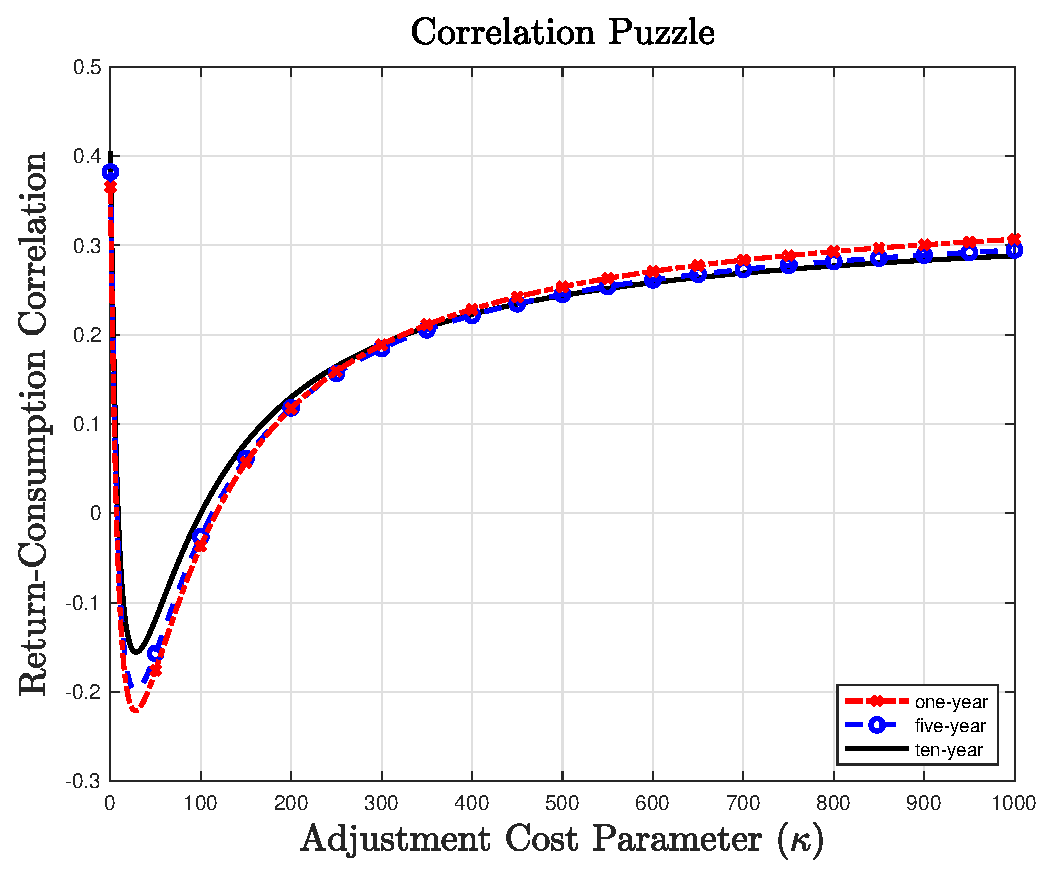
\includegraphics[width=.3\textwidth]{figures/FigProdCorrpuzzle.eps} &
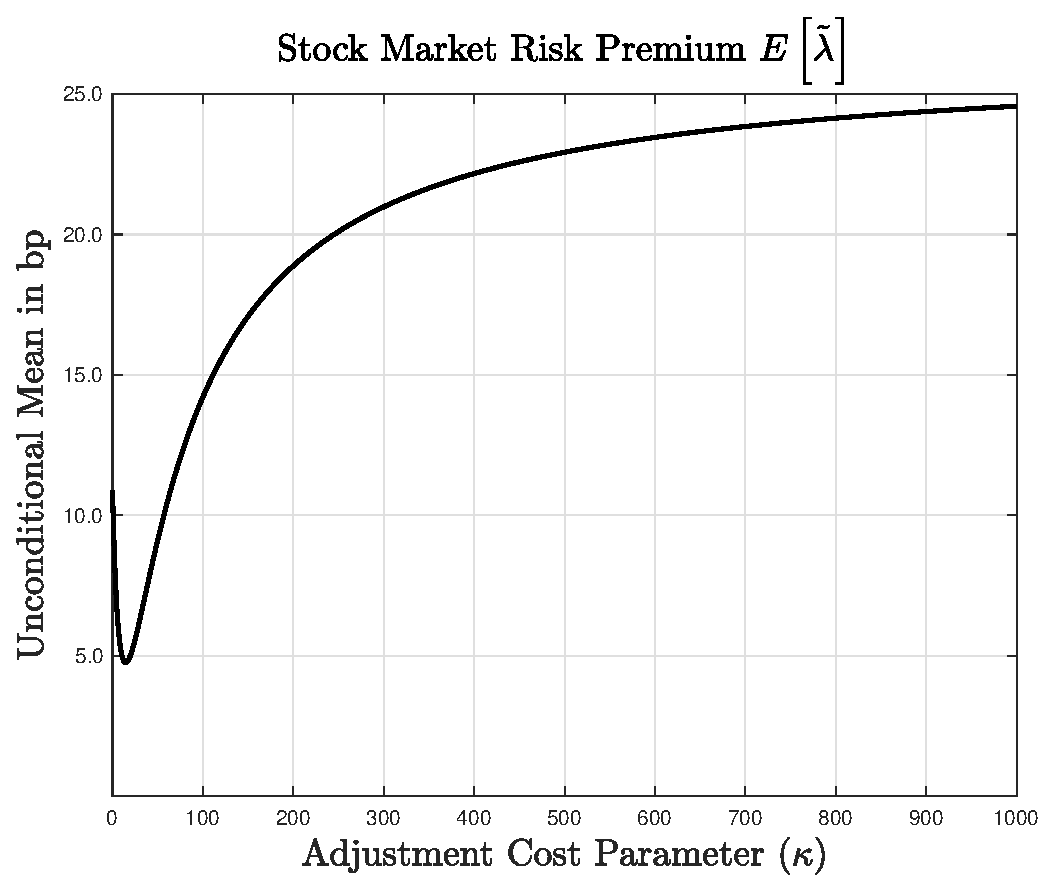
\includegraphics[width=.3\textwidth]{figures/FigProdRP.eps} &
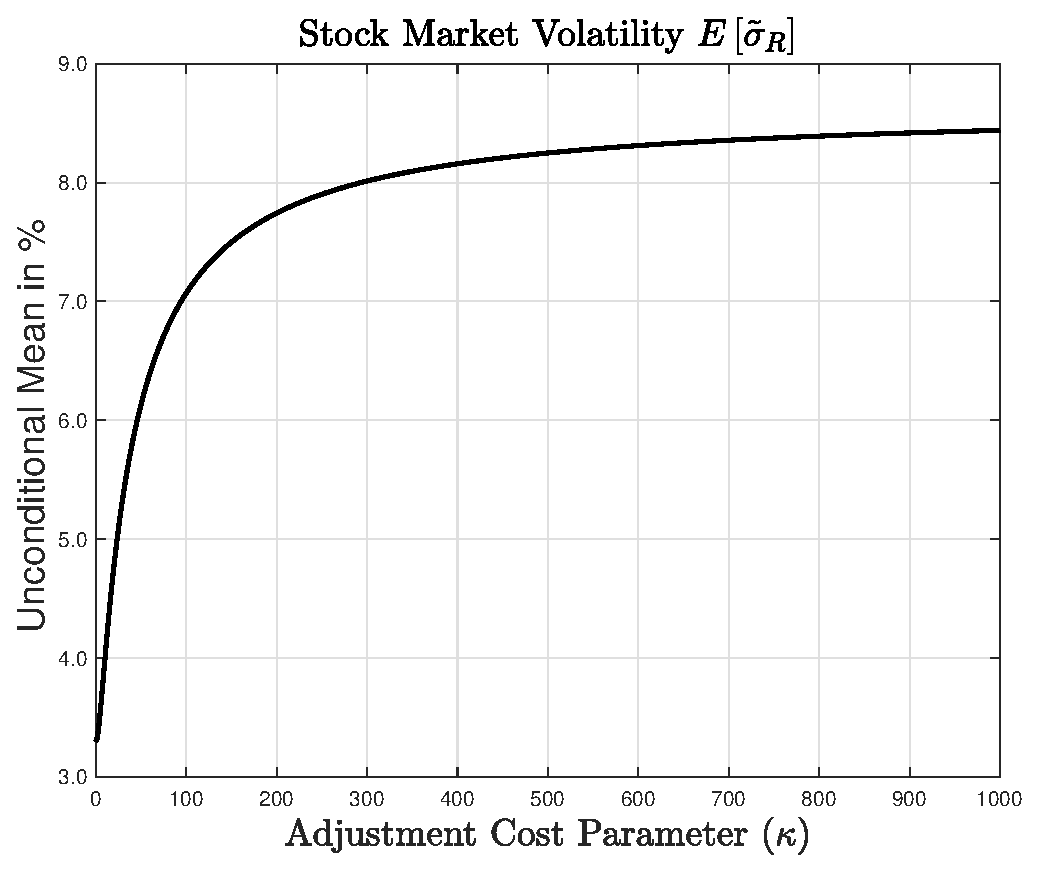
\includegraphics[width=.3\textwidth]{figures/FigProdStdevS.eps}  \\
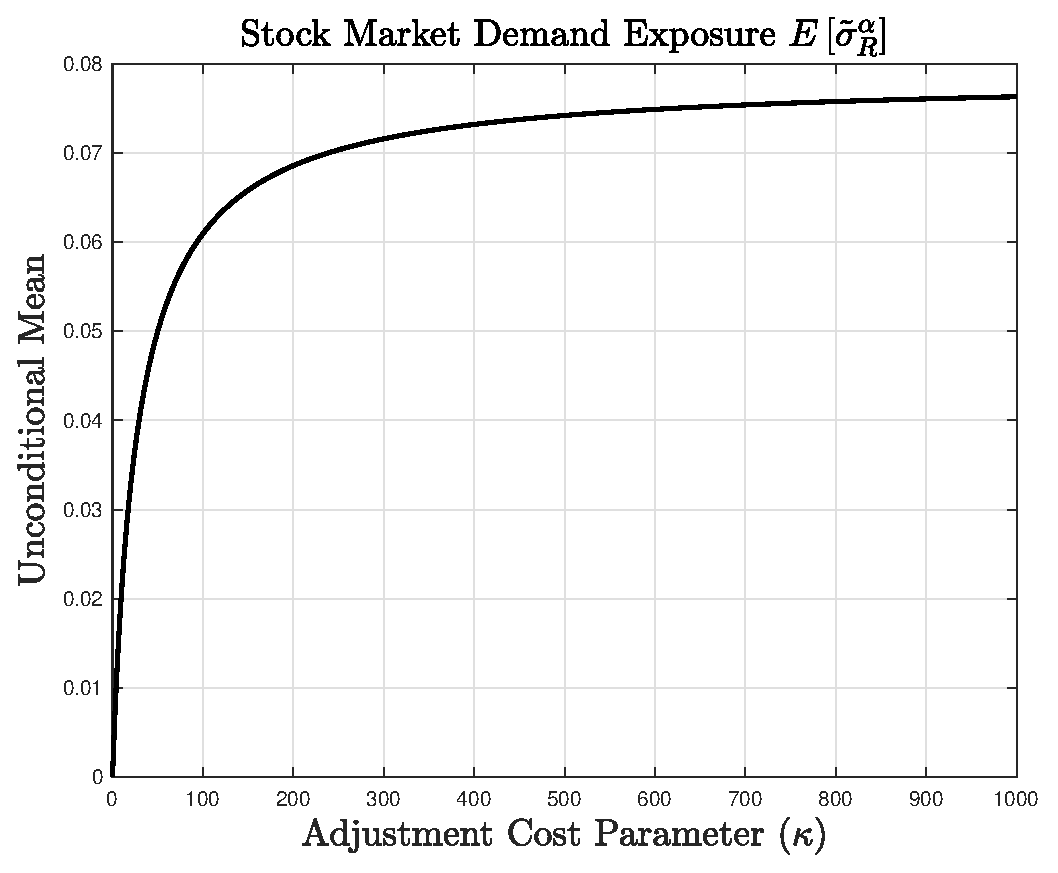
\includegraphics[width=.3\textwidth]{figures/FigProdsigalpS.eps}  &
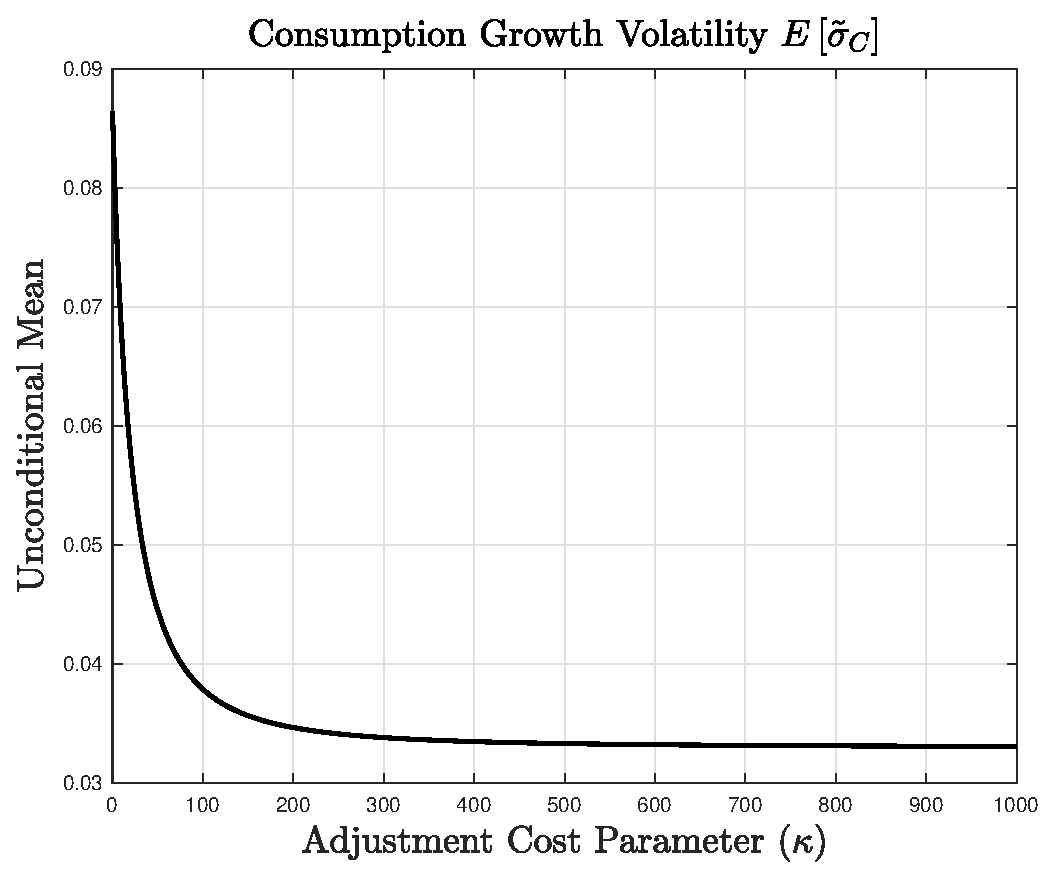
\includegraphics[width=.3\textwidth]{figures/FigProdStdevC.eps} &
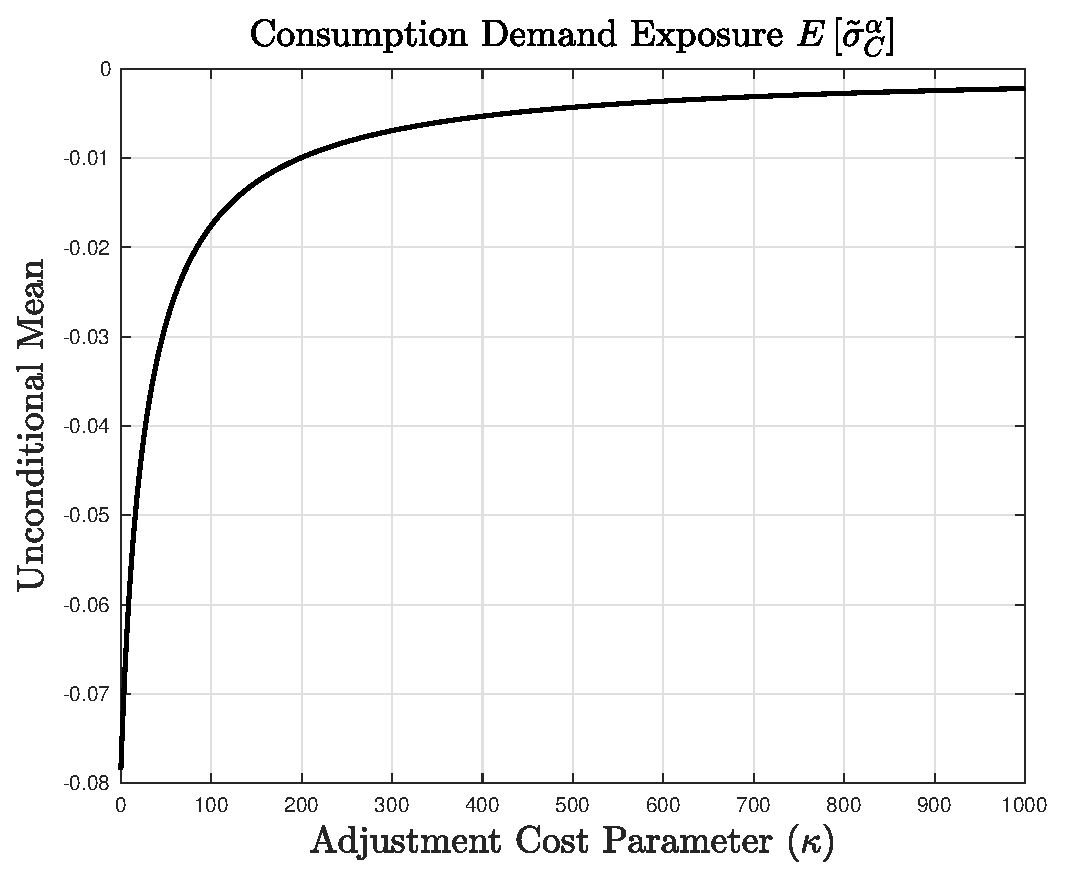
\includegraphics[width=.3\textwidth]{figures/FigProdsigalpC.eps} 
\end{tabular}
\caption{\emph{Demand disagreement in a production model.} \footnotesize{The graphs show the unconditional mean of the return-consumption correlation, the stock market risk premium, the stock market volatility, the stock market demand exposure, the consumption growth volatility, and the consumption demand exposure as a function of the adjustment cost parameter $\kappa$. The summary statistics are based on one million years of monthly observations for each value of $\kappa$.}} \label{fig:prod}
\end{figure}

In contrast to consumption, demand shocks are good news for the stock markets as they lower discount rates. Hence, the unconditional mean of the stock market's exposure to demand shocks is positive as in the exchange economy which we show with the bottom left graph of Figure \ref{fig:prod}. While both consumption growth and stock returns have the same exposure to the productivity of capital they have different exposure to demand shocks. The top left graph shows that this leads to a low correlation between stock returns and consumption growth, that in contrast to an exchange economy, may even be negative. Interestingly, the risk premium for demand shocks is still positive even though aggregate consumption loads negatively on them. The intuition is the same as in the baseline model with the exception that the negative loading partly offsets it. However, it is not strong enough to completely offset the effect, and therefore the risk premium is positive. 


	
	




\section{Wealth Shares}\label{secIA:WealthShares}

There are two state variables in our demand disagreement model: (i) the exogenous fraction of newborn patient investors $\alpha_t$ and (ii) the endogenous consumption share of patient investors $f_t$. Instead of the consumption share we could have also used the wealth share of patient investors as the endogenous state variable. Specifically, the wealth share of patient and impatient investors is
\begin{align*}
	f^W_t &= \frac{1}{W_t} \int_{-\infty}^t \nu  e^{-\nu(t-s)}    \alpha_s W_{s,t}^a \: ds =   \frac{f_t}{\beta^a_t} = \frac{1}{1 + \frac{\nu+\rho_a}{\nu+\rho_b} \frac{1-f_t}{f_t}}. 
\end{align*}
and
\begin{align*}
	1-f^W_t  = \frac{1}{W_t} \int_{-\infty}^t \nu  e^{-\nu(t-s)}   (1-\alpha_s) W_{s,t}^b \: ds   =  \frac{1-f_t}{\beta^b_t}
	= \frac{1}{1 + \frac{\nu+\rho_b}{\nu+\rho_a} \frac{f_t}{1-f_t}},
\end{align*}
respectively. The left graph of Figure \ref{fig:WealthShare} shows the wealth share of patient investors and the right graph shows the consumption share for comparison.  
\begin{figure}[htbp]
\centering
\vspace{0.1in}
\begin{tabular}{cc}
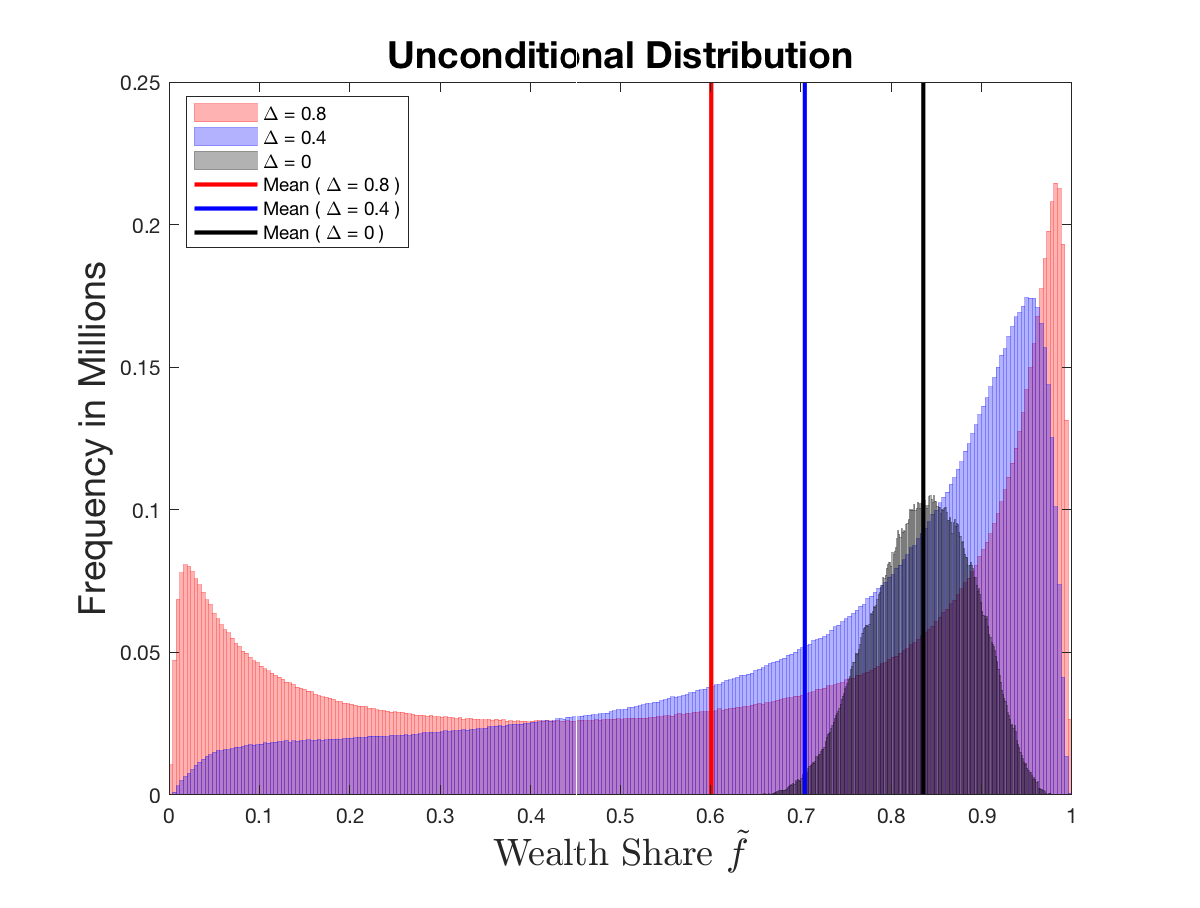
\includegraphics[width=.4\textwidth]{figures/ftWhist.eps} &
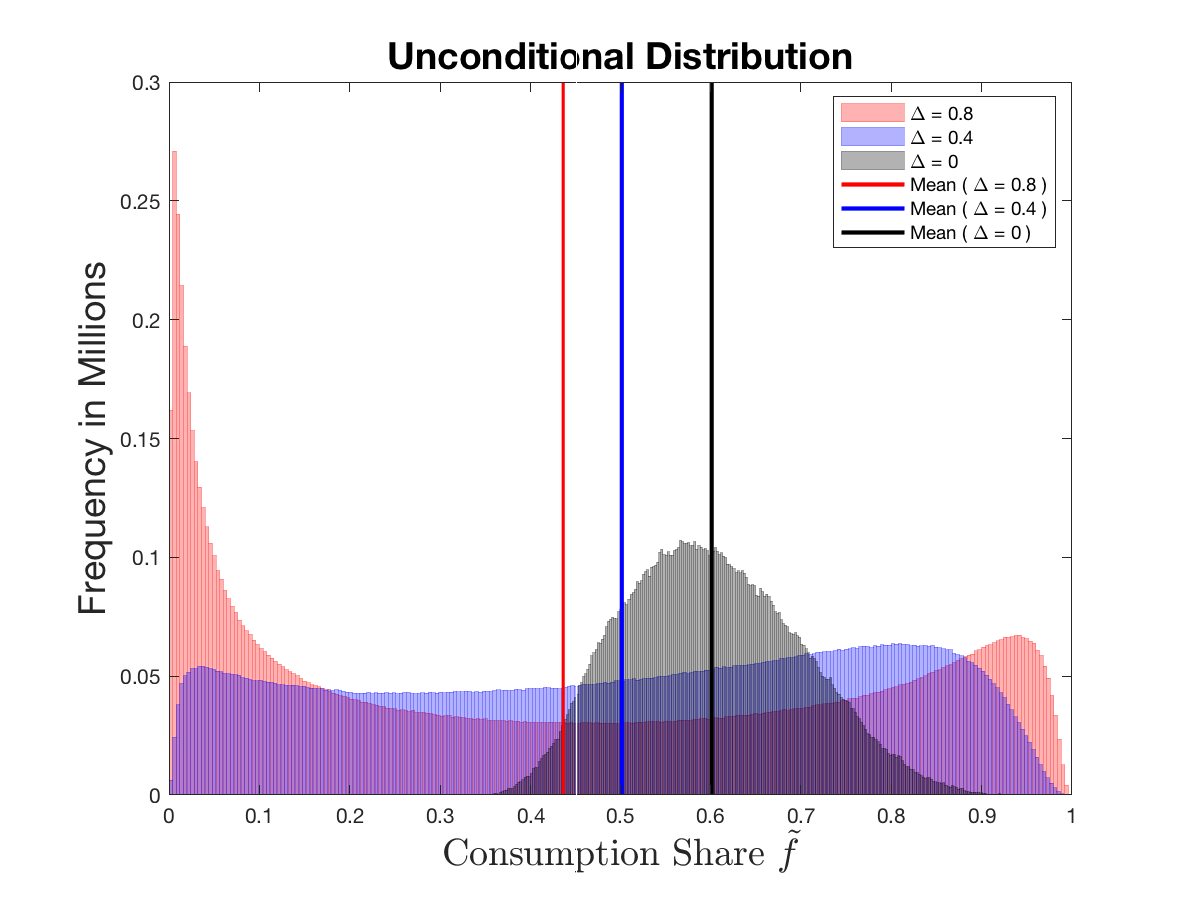
\includegraphics[width=.4\textwidth]{figures/ftHist.eps} \\
\end{tabular}
\caption{\textbf{The Wealth/Consumption share.} \footnotesize{The left graph shows the unconditional distribution of the wealth share $\tilde{f}^W$ and the right graph shows the unconditional distribution of the consumption share of patient investors $\tilde{f}$. The histograms are based one million years of monthly observations for each value of disagreement $\Delta$.  In this example the parameters are based on the alternative calibration with $\rho^a = 0.001$ and $\rho^b = 0.05$}} \label{fig:WealthShare} 
\end{figure}





\section{Correlation Puzzle}
As discussed in the paper, there is a low correlation between returns and fundamentals such as dividends, consumption and output, i.e., the correlation puzzle.  Our demand disagreement model can reconcile the low correlation between output growth and stock market returns and it leads to no correlation between   output growth and both the risk-free rate and trading volume. Specifically, Figure \ref{fig:CorrelationPuzzle} shows the correlation between stock market returns and aggregate consumption for the one, five, and ten year horizon as a function of disagreement $\Delta$.  The figure shows that without disagreement, the correlations are close to one. Hence, demand shocks alone are not sufficient to solve the correlation puzzle.  When disagreement $\Delta$ increases, then the correlation decreases at an increasing rate, and thus for reasonable $\Delta$, we get correlations comparable to the ones we see in the data.  

\begin{figure}[H]
\begin{center}
       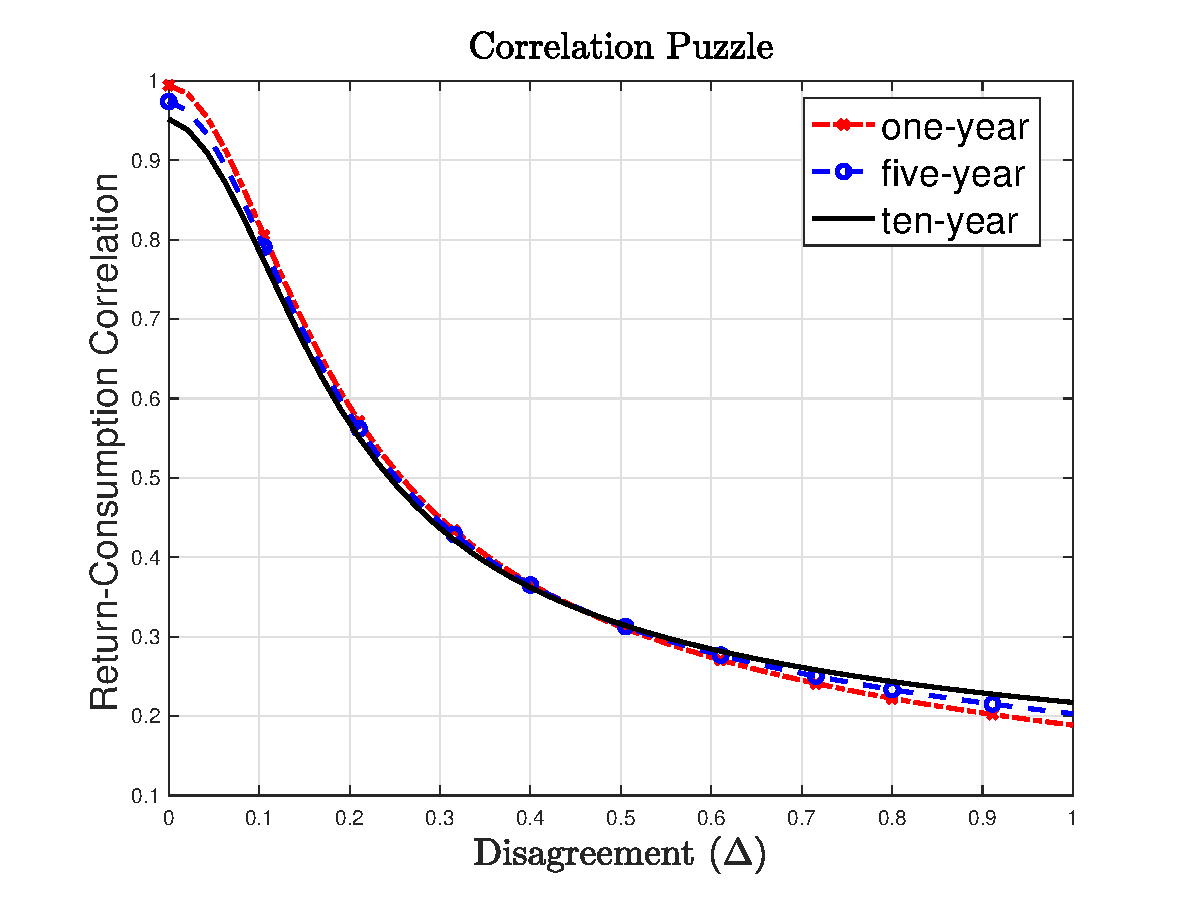
\includegraphics[height=6cm]{figures/CorrelationPuzzle2DEL.eps}  
     \captionsetup{labelformat=andtable}
     \end{center}
\renewcommand\thetable{1}
\caption{\textbf{Correlation puzzle.} \footnotesize{The figure shows the unconditional correlation between stock market returns and aggregate consumption for a one, five and ten year horizon as a function of disagreement $\Delta$. The correlations are based on one million years of monthly observations. In this example the parameters are based on the alternative calibration with $\rho^a = 0.001$ and $\rho^b = 0.05$ }} \label{fig:CorrelationPuzzle} 
\end{figure}

What is the economic intuition for this low correlation in our model? Suppose there are no demand shocks, then the price dividend ratio is constant and stock market returns are perfectly correlated with output shocks. When there are commonly perceived demands shocks, then the price dividend ratio is stochastic but its dynamics are locally deterministic; hence short term correlations between stock market returns and consumption are close to one. The correlation is $0.95$ when measured over ten years and, thus, the indirect effect of the demand shock through the drift of the consumption share is quantitatively small.  The indirect effect is small because heterogeneous time preferences only lead to different consumption-savings rates.   In contrast, when agents have different beliefs about demand shocks, they engage in speculative trade, thus changing their consumption-saving rates and portfolio compositions. Demand shocks, which are by assumption independent of output shocks, lead to shocks to the price-dividend ratio, the risk free rate, the volatility and risk premium of the stock market, and trading volume. Hence, demand disagreement breaks the tight link between shocks to output growth and stock market returns and solves the correlation puzzle.   Similar to the risk-free rate, disagreement and the resulting trade in the stock market is purely driven by demand shocks and, hence, the correlation between macroeconomic fundamentals and both the risk-free rate and trading volume, which is also low in the data, is by construction zero.\footnote{It is straightforward to increases this correlation by adding disagreement about output growth.} 

From the above discussion it is clear that in our model the correlation puzzle and the disagreement correlation puzzle are closely related -- all disagreement in asset prices are due to demand disagreement  and without demand disagreement the model cannot generate sufficient disconnect between asset prices and macroeconomic fundamentals to replicate the correlation puzzle. 

\section{Price-dividend ratio and return predictability}
 Given that the valuation ratio is linear in the consumption share, the price-dividend ratio (or wealth-consumption ratio) predicts returns in our model. The left graph of Figure \ref{fig:StockMarketPredictability} shows that the slope coefficient of the predictability regression is negative and the right graph shows that the $R^2$ is increasing with the predictability horizon. Specifically, the slope is strictly decreasing and the $R^2$ is strictly increasing with disagreement. The intuition is straightforward when looking at the right graph of Figure \ref{fig:VolaRiskPremium2f}. It shows that the equity premium is decreasing with the consumption share and, thus, decreasing with the price-dividend ratio except for very low or very high consumption share realizations which do not occur often.  Moreover, the sensitivity of the equity premium to changes in the price-dividend ratio increases with disagreement and vanishes if there is no disagreement because in this case the equity premium is constant.  Interestingly, we expect the predictive relation to change signs in times of very high or low stock market valuations.\footnote{In the Internet Appendix we show that the model is also consistent with the Black's ``Leverage'' effect, i.e., the conditional volatility is negatively correlated with stock market returns.}

\begin{figure}[H]
\centering
\begin{tabular}{cc}
\includegraphics[width=.4\textwidth]{figures/PDregressionSlope2Dis.eps} &
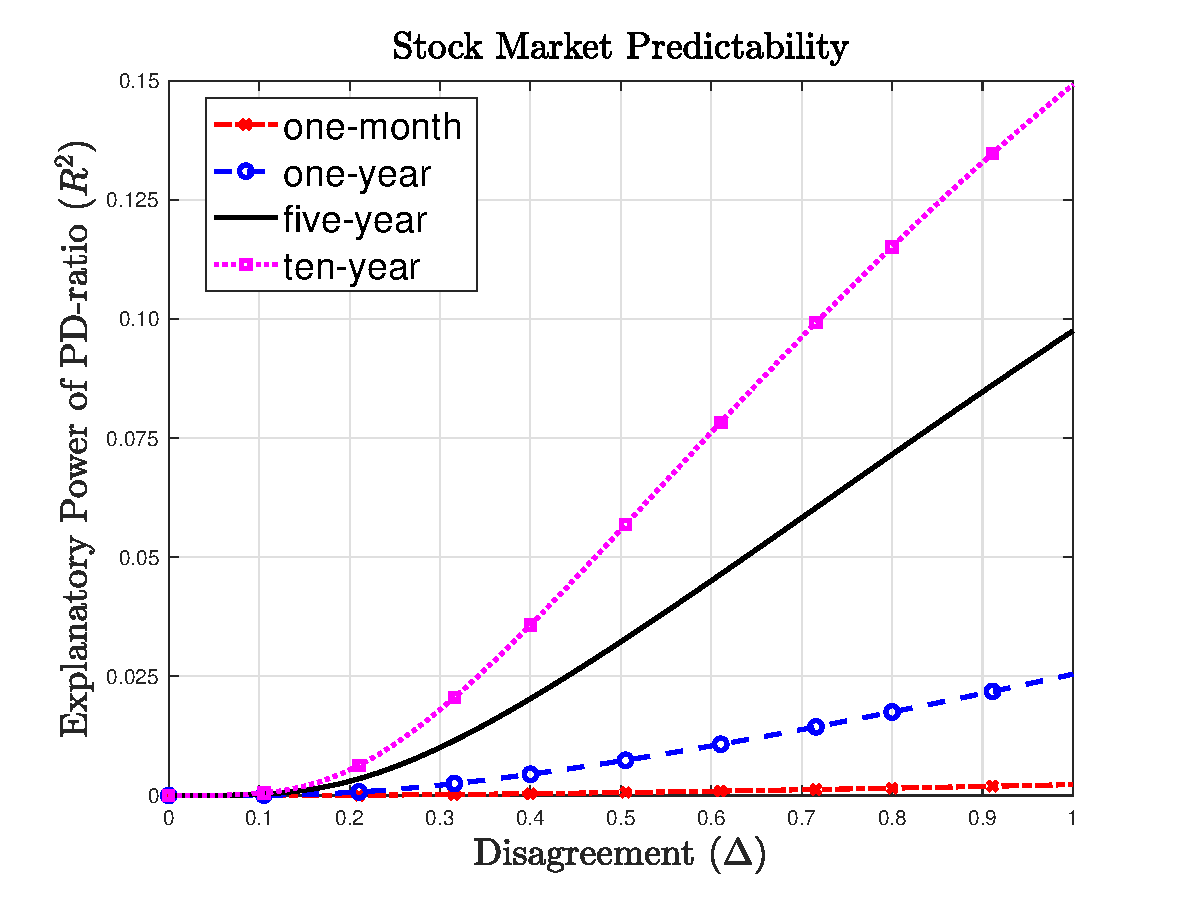
\includegraphics[width=.4\textwidth]{figures/PDregressionRsq2Dis.eps} \\  
\end{tabular}
\caption{\textbf{Stock Market Predictability.}  \footnotesize{The left graph shows the slope and the right graph shows the $R^2$ for the price-divided regressions $Rx_{t,t+\tau} = a + b \phi_t + \epsilon_{t+\tau}$, where $Rx_{t,t+\tau}$ is the excess stock market return from $t$ to $t+\tau$. An increase in the price-dividend ratio lowers expected stock market returns in excess of the risk-free rate. Moreover, the economic significance and explanatory power of this predictive regression is increasing in disagreement.  The slope and $R^2$ are averages based on one million years of monthly observations for each value of disagreement $\Delta$. In this example the parameters are based on the alternative calibration with $\rho^a = 0.001$ and $\rho^b = 0.05$}}  
\label{fig:StockMarketPredictability} 
\end{figure}

\ref{fig:VolaRiskPremium2f} show.
\begin{figure}[H]
\centering
\vspace{0.1in}
\begin{tabular}{cc}
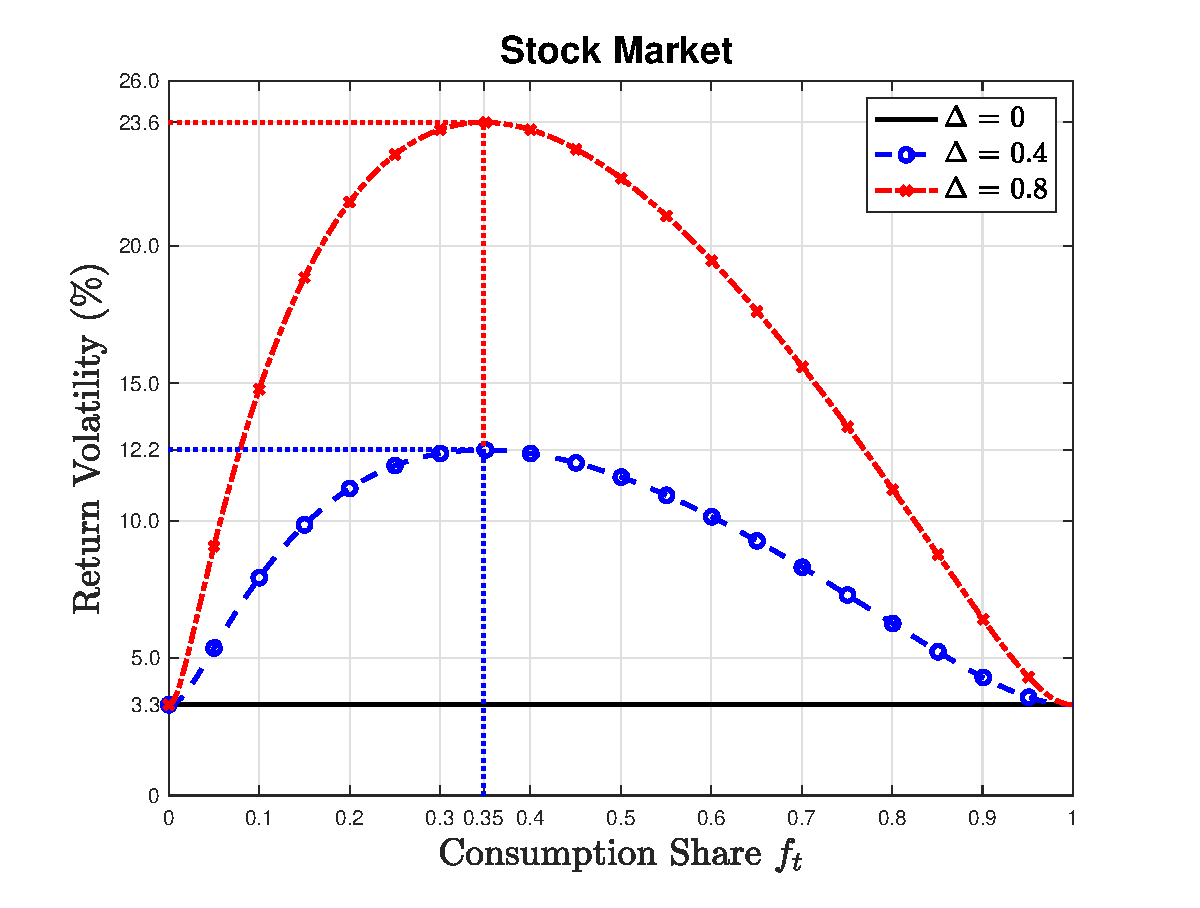
\includegraphics[width=.45\textwidth]{figures/StockMarketVola2f.eps} &
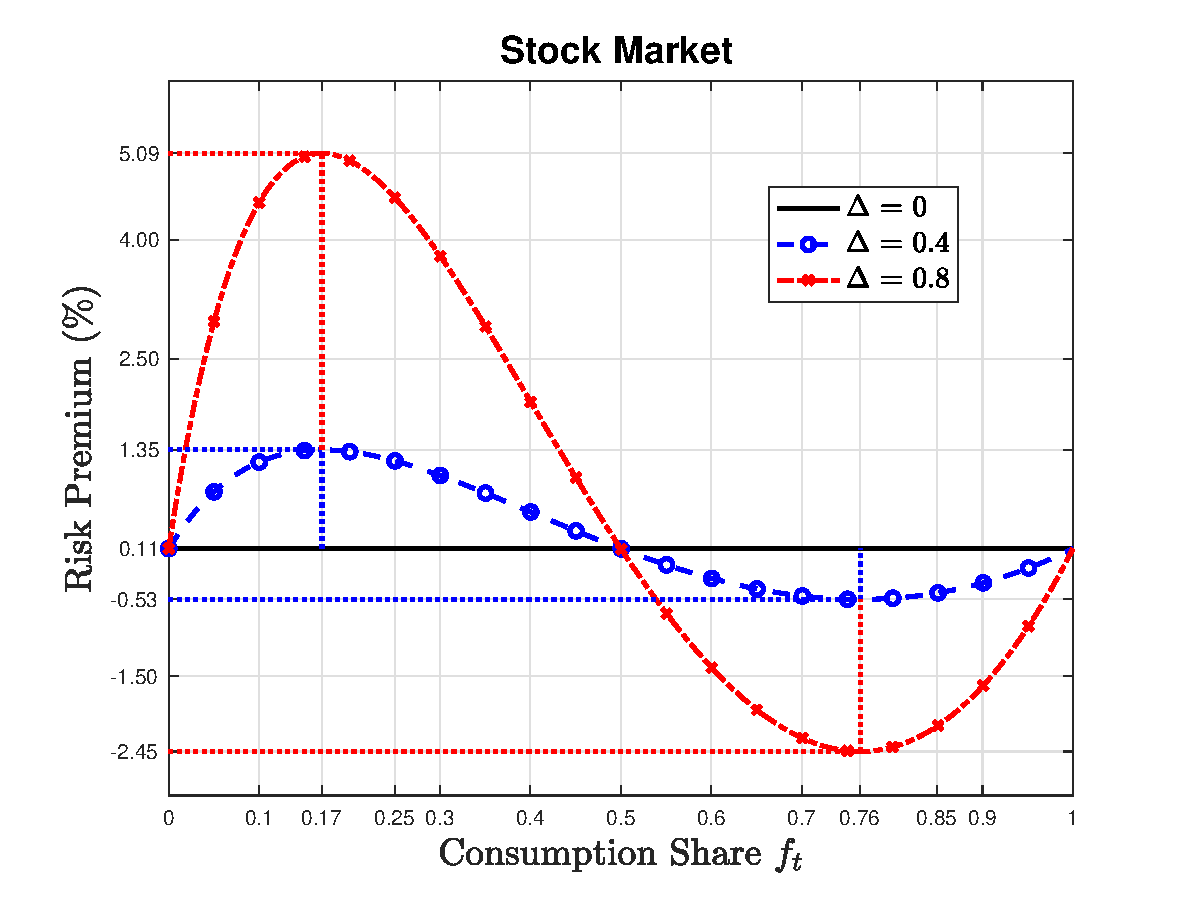
\includegraphics[width=.45\textwidth]{figures/StockMarketRiskPremium2f.eps}
\end{tabular}
\caption{\textbf{Conditional stock market volatility and risk premium.} \footnotesize{The left graph shows stock market volatility and the right graphs shows the equity premium conditional on the consumption share $f_t$ for different disagreement $\Delta$. Disagreement leads to stochastic stock market volatility in excess of output growth volatility and to a stochastic equity premium that is positive if impatient cohorts consume more out of output and negative if patient cohorts consume more out of output. In this example the parameters are based on the alternative calibration with $\rho^a = 0.001$ and $\rho^b = 0.05$}} \label{fig:VolaRiskPremium2f} 
 \end{figure}

\section{Changes in demand risk exposure}
Trading volume is difficult to define because it depends on the asset structure. Therefore, we introduce a measure that is independent of the asset structure but nevertheless captures the effects of disagreement on trading volume with the caveat that is not directly comparable to trade in a specific asset. Specifically, Definition \ref{Def:TotExpsure} below introduces the concept of excess exposure to supply and demand shocks. It basically captures how investors' optimal portfolios deviate from two-fund separation. Based on this measure, we define trading volume as variations of excess exposure and determine it in Proposition \ref{prop:TradingVolume} below. This measure captures the notion that large changes in excess exposure have to come from changes in underlying asset positions. 

 \begin{defn}[Excess Exposure]\label{Def:TotExpsure}
 Let $\mu^{W,i}_{s,t}$ denote the drift, $\sigma^{W,i}_{Y,s,t}$ the supply shock (output) exposure, and $\sigma^{W,i}_{\alpha,s,t}$ the demand shock exposure of a patient (type i=a) and impatient (type i=b) investor born at time $s$ with total wealth dynamics
 \begin{equation} \label{eq:totwealthind}
 \frac{dW^i_{s,t}}{W^i_{s,t}} = \mu^{W,i}_{s,t} \:  dt + \sigma^{W,i}_{Y,s,t} \: dZ_{Y,t}  
	+ \sigma^{W,i}_{\alpha,s,t} \: dZ_{\alpha,t}.
\end{equation}
Investors' supply and demand shock exposure in excess of their exposure to both shocks trough the value of their endowment stream is defined as 
\begin{align}\label{eq:XE_Y}
   \text{XE}_{Y,t} &= \int_{-\infty}^{t} \nu e^{\nu \left(t-s\right)}\left(\alpha_s \beta^{W,a}_{s,t} \lvert  \sigma^{W,a}_{Y,s,t} \rvert 
 +\left(1-\alpha_s\right) \beta^{W,b}_{s,t} \lvert \sigma^{W,b}_{Y,s,t}  \rvert \right)ds  -  \lvert \sigma^{Y}_{R,t}\rvert \\
  \text{XE}_{\alpha,t} &= \int_{-\infty}^{t} \nu e^{\nu \left(t-s\right)}\left(\alpha_s \beta^{W,a}_{s,t}  \lvert \sigma^{W,a}_{\alpha,s,t} \rvert 
 +\left(1-\alpha_s\right)\beta^{W,b}_{s,t} \lvert  \sigma^{W,b}_{\alpha,s,t}  \rvert \right)ds -  \lvert \sigma^{\alpha}_{R,t}\rvert,
\end{align} 
respectively, where $\beta^{W,i}_{s,t} =  W^i_{s,t}/ W_t$ denotes the individual wealth share of a type i investor. 
\end{defn}
We derive the excess exposure to supply and demand shocks in the next proposition.
\begin{prop}[Excess Exposure]\label{prop:Exposure}
 The individual supply shock exposure, demand shock exposure, and drift of investors' wealth $W^i_{s,t}$ is $ \sigma^{W,i}_{Y,s,t} = \sigma_Y$,  $\sigma^{W,i}_{\alpha,s,t} = \theta_{\alpha,t}^i$, and $\mu^{W,i}_{s,t} =  r_t +\sigma_Y^2+\left( \theta_{\alpha,t}^i \right)^2 -\rho^i$, respectively. 
There is no excess exposure to supply shocks, that is,  is $\text{XE}_{Y,t} =0$ but there is excess exposure to demand shocks. Specifically,
 \begin{equation}\label{eq:XEdemand}
	\text{XE}_{\alpha,t}= 2 \frac{\phi_b}{\phi_t}  f_t  \left(1-f_t\right) \Delta = 2 \frac{\phi_b}{\phi_a-\phi_b} \sigma^{\alpha}_{R,t} \geq 0. 
\end{equation}
\end{prop} 
There is no disagreement on supply shocks and consequently investors do not speculate on it. Hence, investors' fractions of wealth invested in the market portfolio are equally exposed to supply shocks and, thus, there is no excess exposure to these shocks. If investors disagree on demand shocks, then they trade on this disagreement and by doing so invest different fractions of their wealth in the market portfolio even though they have the same risk preferences. The more they deviate from two-fund separation, the larger the excess exposure to demand shocks.   Equation (\ref{eq:XEdemand}) shows that this exposure is  proportional to the stock market loading onto demand shocks and, thus, inherits all properties of the stock market volatility. 

We define trading volume or trading intensity as the square root of the instantaneous quadratic variation of excess exposure to demand shocks. This is similar to the continuous time literature that typically use the quadratic variation of portfolio policies as a measure of the trading intensity (e.g. \citeasnoun{grossman-zhou:96}, \citeasnoun{longstaff-wang:12}, and \citeasnoun{EhlingHeyerdahlLarsen2016}).  

\begin{prop}\label{prop:TradingVolume}
 Let $QV_{t,T}$ denote the quadratic variation of excess demand risk exposure. Specifically,
 \begin{equation}
  QV_{t,T} = \int_t^{T} d\text{XE}_{\alpha,u} d\text{XE}_{\alpha,u} = \int_t^{T} \left(\text{TVol}_u\right)^2 \: du.
 \end{equation}
 Then $\text{TVol}_t$ denotes the trading volume or trading intensity. Specifically, 
\begin{equation}\label{eq:TVol}
	\text{TVol}_t = 2\phi^b \Delta^2  \frac{f_t (1-f_t) }{\phi_t^2} \lvert \phi^B \left(1-f_t\right)^2 - \phi^A f_t^2   \rvert.
\end{equation}
\end{prop}

\begin{figure}[H] 
\centering
\begin{tabular}{cc}
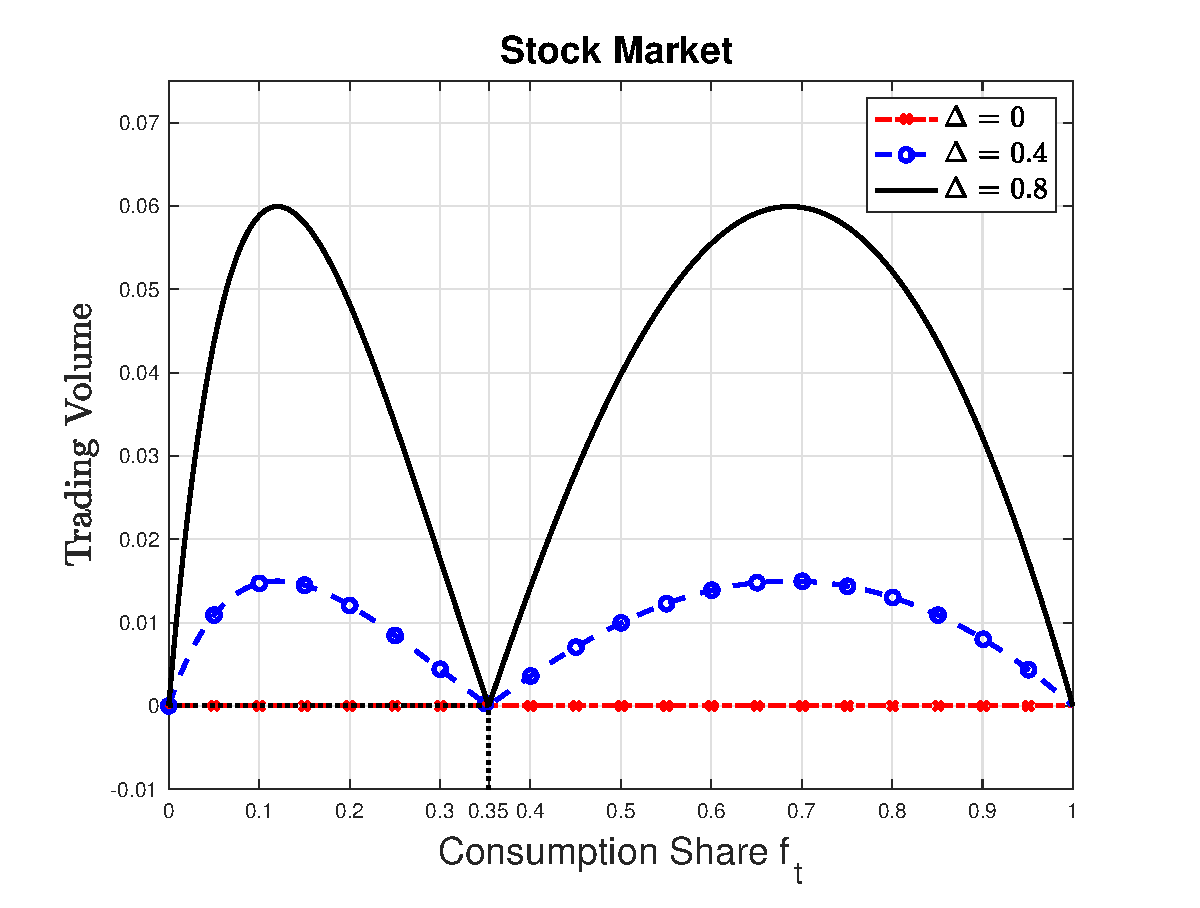
\includegraphics[width=.4\textwidth]{figures/TradingVolume2f.eps} &
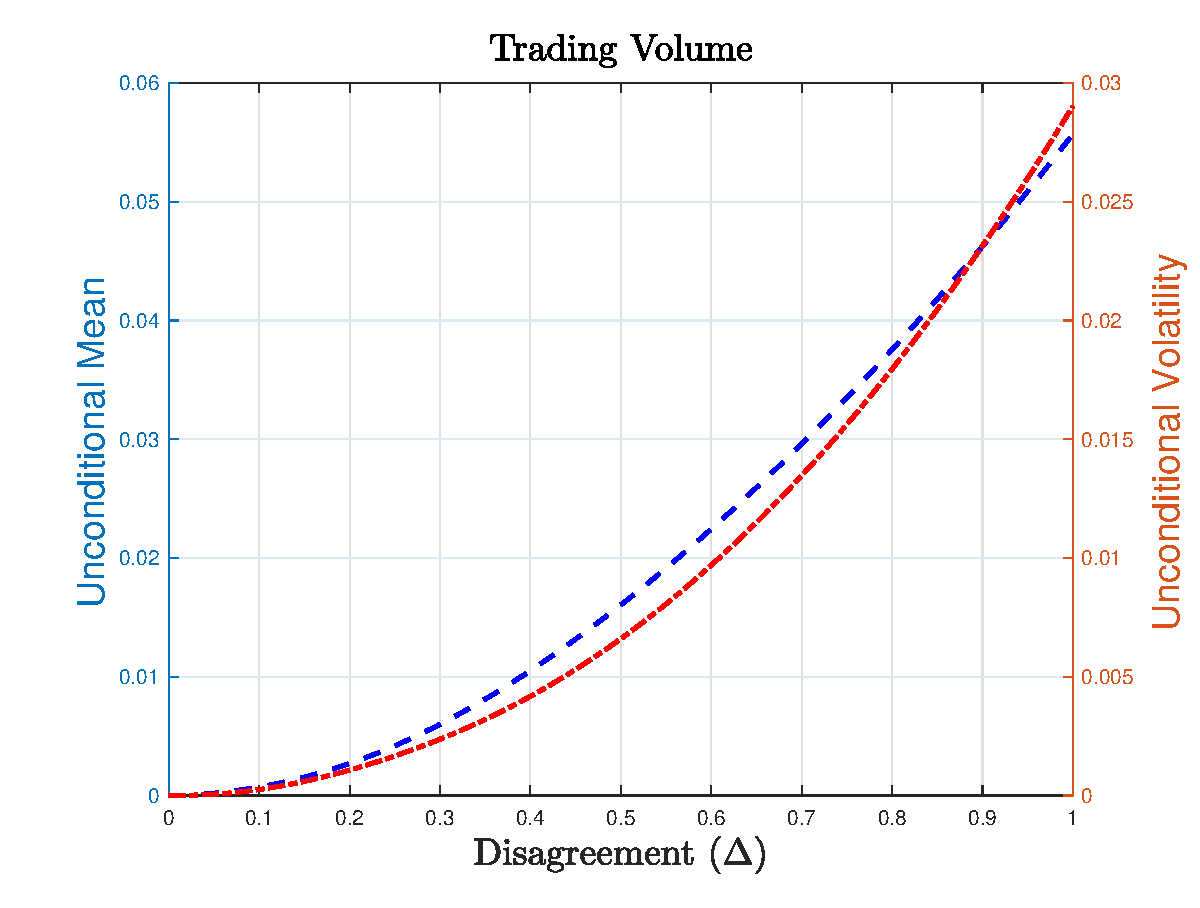
\includegraphics[width=.4\textwidth]{figures/TradingVolume2DELmeanvol.eps} 
\end{tabular}
\caption{\emph{Trading volume or trading intensity.} \footnotesize{The left graph shows trading volume/intensity as a function of the consumption share $f_t$ for different disagreement $\Delta$ and the right graph shows the unconditional mean and volatility of it as a function of disagreement $\Delta$. Trading volume is a non monotone function of the consumption share but both its mean and volatility are strictly increasing in disagreement. The unconditional statistics are based on one million years of monthly observations. In this example the parameters are based on the alternative calibration with $\rho^a = 0.001$ and $\rho^b = 0.05$}}   \label{fig:tradingf} 
\end{figure}

The left graph of Figure \ref{fig:tradingf} shows that trading volume is a non monotone function of the consumption share that is increasing in disagreement. Moreover, the right graph of Figure \ref{fig:tradingf} shows that the unconditional mean and volatility of trading volume is strictly increasing in disagreement. 

\section{Black's ``Leverage'' Effect}

One of the most well-established empirical regularities of equity markets is the negative correlation between the return of stocks and their volatility. In a seminal paper, \citeasnoun{Black1976} provides financial leverage as compelling explanation for this phenomenon. While this effect, and the leverage-based explanation, have been empirically confirmed by a number of studies more recent papers show that financial leverage is not the only reason for the negative relation between the return of stocks and their volatility (e.g. \citeasnoun{HasanhodzicLo2011}). %For instance, \citeasnoun{HasanhodzicLo2011} confirm this negative relation for all-equity financed companies. 
In our model, the negative relation between the stock market return and its volatility is due to the time-variation in consumption/wealth shares.     


We derive the local correlation between stock market returns and changes in stock market volatility in Proposition \ref{prop:LEV}. This correlation is usually set to be negative in the derivatives literature (e.g. \citeasnoun{Heston1993}) and it is endogenous in our demand disagreement model. Specifically, we know from the paper that the stock market volatility is strictly increasing in the consumption share until it attains its maximum at $f_{\sigma_R}^{\text{max}}=0.35$ and it is strictly decreasing after that. Positive shocks to the consumption share are good news for the stock market and, thus, the correlation between stock returns and their volatilities is positive for low consumption shares and negative otherwise.  The left plot of Figure \ref{fig:BlackLeverageEffect} provides a graphic illustration of this correlation conditional on the consumption share for different disagreement $\Delta$.  


\begin{prop}[Black's ``Leverage'' Effect]\label{prop:LEV}
Let $f_{\sigma_R}^{\text{max}}$ denote the consumption share value that maximizes the conditional stock market volatility. The local correlation between the return on the stock market and its volatility in equilibrium is
\begin{align}\label{eq:MP_Demand_Sig}
  	\rho_{LE}(f_t) = \text{corr} \left (dR_t, \frac{d\sigma_{R,t}}{\sigma_{R,t}} \right)
  	&= \left \lbrace \begin{array}{lcl}
  		\frac{\sigma^{\alpha}_{R,t}}{\sigma_{R,t}}  
  		& \text{if} & f_t < f_{\sigma_R}^{\text{max}} \\
  		0 & \text{if} & f_t = f_{\sigma_R}^{\text{max}} \\
  		-\frac{\sigma^{\alpha}_{R,t}}{\sigma_{R,t}}  
  		& \text{if} &f_t >f_{\sigma_R}^{\text{max}}. 
  		\end{array} \right. 
\end{align}
\end{prop}
The right graph of Figure \ref{fig:BlackLeverageEffect} shows the unconditional mean of the correlation $\rho_{LE}\left(\tilde{f}\right)$ as a function of disagreement $\Delta$. This correlation is zero without disagreement and becomes negative with low disagreement because in this case there is a low probability of high consumption share realizations of impatient investors. This probability increases when we increase disagreement and, thus, the correlation also decreases for high $\Delta$ after hitting its minimum around $-0.54$.    


\begin{figure}[H]%[htbp]
\centering
\begin{tabular}{cc}
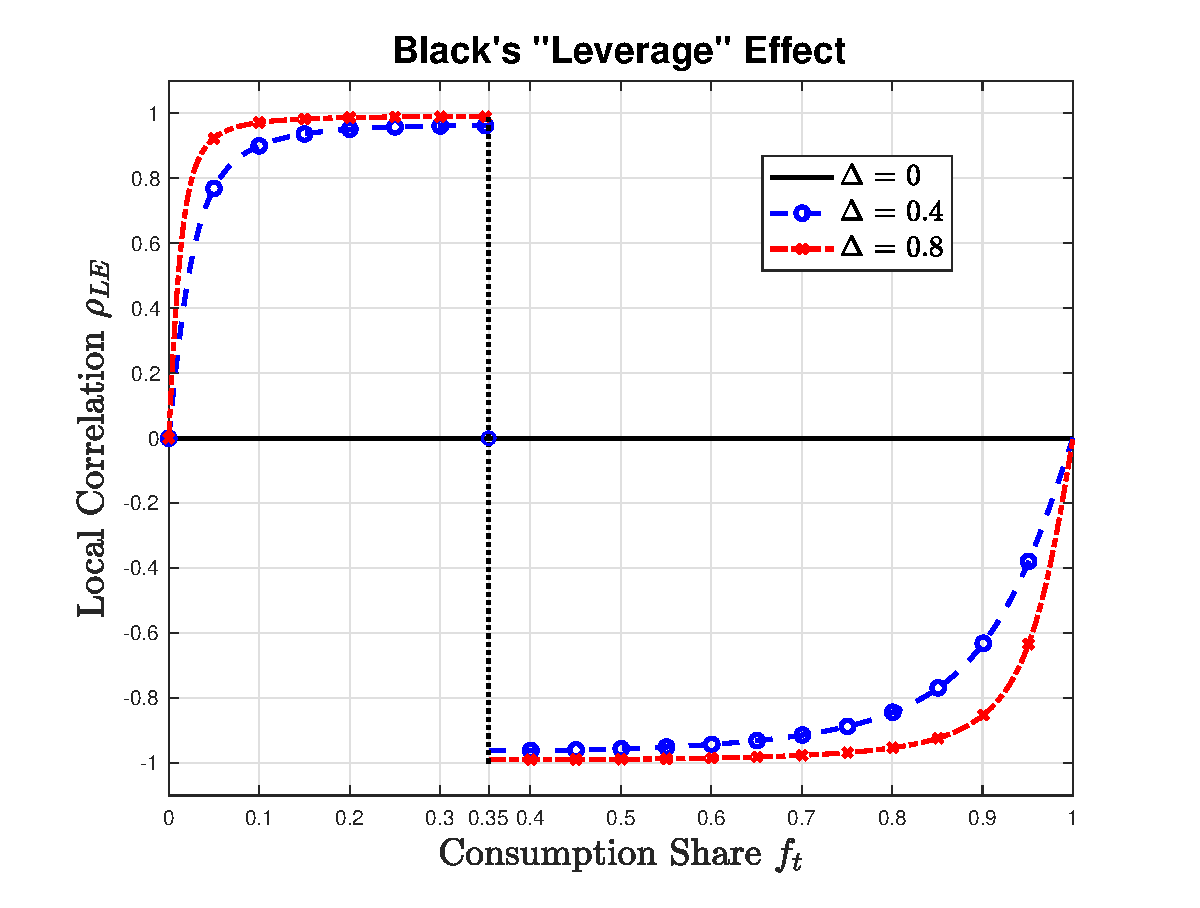
\includegraphics[width=.4\textwidth]{figures/BlackLeverageEffect2f.eps} &  
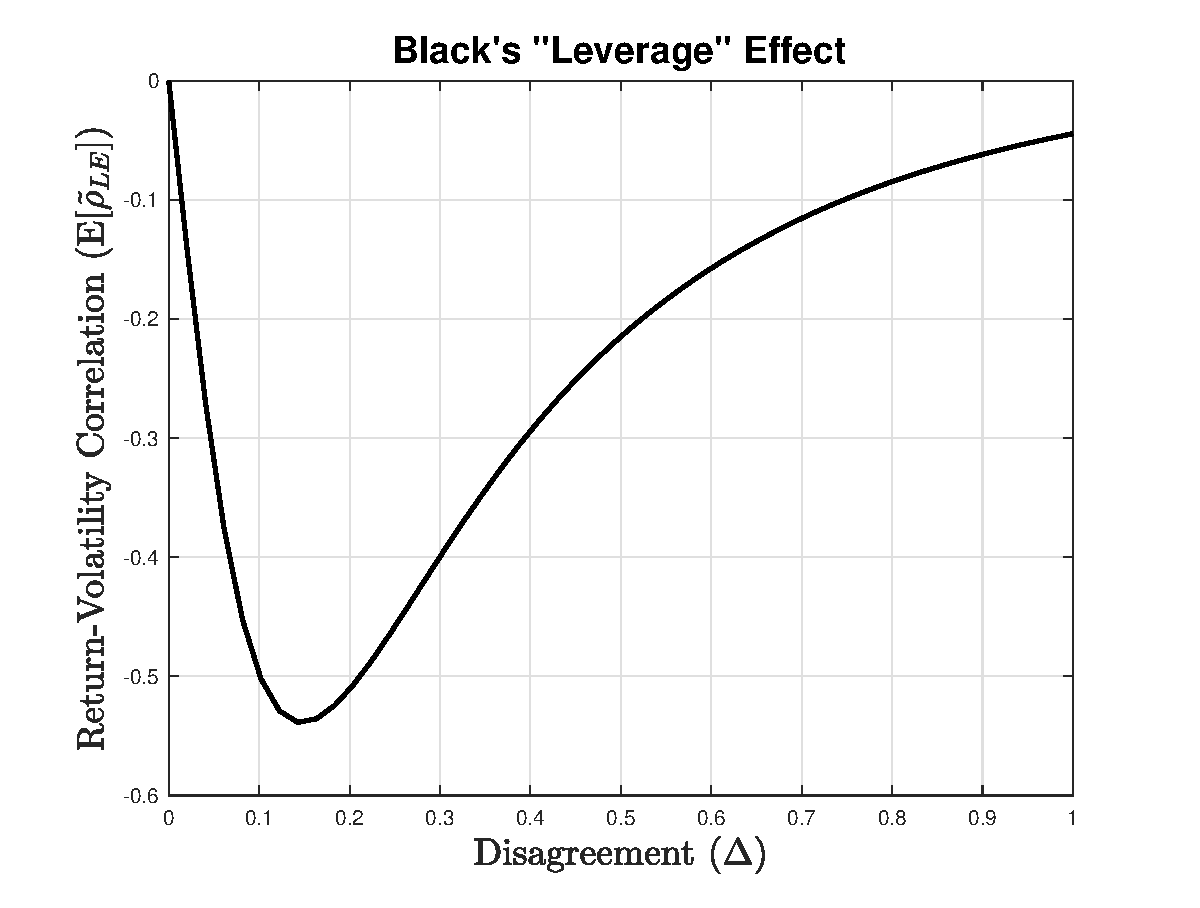
\includegraphics[width=.4\textwidth]{figures/BlackLeverageEffect2DEL.eps} \\ 
\end{tabular}
\caption{\textbf{Black's ``Leverage" Effect.}  \footnotesize{The left graph shows the local correlation between the stock market return and its volatility as a function of the consumption share $f_t$ for different disagreement $\Delta$ and the right graph shows the unconditional distribution of this correlation as a function of disagreement $\Delta$.   The unconditional statistic is based on one million years of monthly observations for each value of disagreement $\Delta$. In this example the parameters are based on the alternative calibration with $\rho^a = 0.001$ and $\rho^b = 0.05$}} 
\label{fig:BlackLeverageEffect} 
\end{figure}



\bibliographystyle{jfe}
\newpage
\bibliography{OLGBeliefsAccepted}\label{references}

\end{document}





